\documentclass{article}



\usepackage{arxiv}

\usepackage[utf8]{inputenc} % allow utf-8 input
\usepackage[T1]{fontenc}    % use 8-bit T1 fonts
\usepackage{hyperref}       % hyperlinks
\usepackage{url}            % simple URL typesetting
\usepackage{booktabs}       % professional-quality tables
\usepackage{amsfonts}       % blackboard math symbols
\usepackage{nicefrac}       % compact symbols for 1/2, etc.
\usepackage{microtype}      % microtypography
\usepackage{lipsum}		% Can be removed after putting your text content
\usepackage{graphicx}
\usepackage{amsmath}
\usepackage{graphicx,caption} % omit figure numbering in supplementary materials

%\usepackage{natbib}
\usepackage{doi}

% The humanities-type option: author-year in-text citation with an alphabetical works cited.
\usepackage[style=apa, sorting=nyt, backend=biber, uniquename=false, uniquelist=true, maxcitenames=5, useprefix, doi=true, isbn=false]{biblatex}
\newcommand*{\bibtitle}{References}
%\setlength\bibitemsep{\baselineskip}
% This makes the bibliography left-aligned (not 'justified') and slightly smaller font.
\renewcommand*{\bibfont}{\raggedright\small}
% Change this to the name of your .bib file (usually exported from a citation manager like Zotero or EndNote).
\addbibresource{library.bib}


\title{Multiple and Dissociable Effects of Sensory History on Working-Memory Performance}

%\date{September 9, 1985}	% Here you can change the date presented in the paper title

\author{ \href{https://orcid.org/0000-0002-0812-6842}{\includegraphics[scale=0.06]{orcid.pdf}\hspace{1mm}Jasper  E.~Hajonides} \\
	Oxford Centre for Human Brain Activity, \\
	University of Oxford, UK\\
	Department of Experimental Psychology, \\
	University of Oxford, UK \\
	%% examples of more authors
	\And
	\href{https://orcid.org/0000-0002-7434-1751}{\includegraphics[scale=0.06]{orcid.pdf}\hspace{1mm}Freek van Ede} \\
	Department of Applied and Experimental Psychology,\\
	Vrije Universiteit, NL
	\AND
	Mark G. Stokes \\
	Department of Experimental Psychology, \\
	University of Oxford, UK \\
	\And
	\href{https://orcid.org/0000-0001-5762-2802}{\includegraphics[scale=0.06]{orcid.pdf}\hspace{1mm}Anna C. Nobre} \\
	Oxford Centre for Human Brain Activity, \\
	University of Oxford, UK\\
	Department of Experimental Psychology, \\
	University of Oxford, UK
	\And
	\href{https://orcid.org/0000-0001-5599-3044}{\includegraphics[scale=0.06]{orcid.pdf}\hspace{1mm}Nicholas E. Myers}\thanks{Corresponding author. E-mail address: Nick.Myers@nottingham.ac.uk} \\
	School of Psychology \\
	University of Nottingham, UK \\ 
	Department of Experimental Psychology, \\
	University of Oxford, UK
}
% Uncomment to override  the `A preprint' in the header
%\renewcommand{\headeright}{Technical Report}
%\renewcommand{\undertitle}{Technical Report}
\renewcommand{\shorttitle}{\textit{bioRxiv} Template}

%%% Add PDF metadata to help others organize their library
%%% Once the PDF is generated, you can check the metadata with
%%% $ pdfinfo template.pdf
\hypersetup{
pdftitle={A template for the bioRxiv style},
pdfsubject={q-bio.NC, q-bio.QM},
pdfauthor={Jasper E.~Hajonides},
pdfkeywords={working memory, biases, neural representations},
}

\begin{document}

\maketitle

\begin{abstract}
Behavioural responses to sensory information are biased by stimulus history. The nature and direction of such serial-dependence biases in performance can differ between experimental settings – both attractive and repulsive biases towards previous stimuli have been observed. How and when these biases arise in the human brain remains largely unexplored. They could occur either via a change in sensory processing itself, post-perceptual maintenance or decision-making processes, or both. Here, we analysed behavioural and magnetoencephalographic data from a working-memory task in which participants were sequentially presented with two randomly oriented gratings, one of which was cued for recall at the end of the trial. Behavioural responses showed evidence for two distinct biases: 1) a within-trial repulsive bias away from previously encoded orientation on the same trial and 2) a between-trial attractive bias towards the task-relevant orientation on the previous trial. Multivariate classification of stimulus orientation revealed that neural representations during stimulus encoding were biased away from the previous grating orientation, regardless of whether we considered the within-trial or the between-trial prior grating orientation – despite opposite effects observed in behaviour. These results suggest that repulsive biases occur at the level of sensory processing and can be overturned at post-perceptual stages to result in attractive biases in behavioural performance. 
\end{abstract}
%
%
%% keywords can be removed
\keywords{working memory \and biases \and neural representations}


\section{Introduction}
Stimulus history modulates performance based on sensory input. The incorporation of recently perceived information is a beneficial strategy within a world that is largely stable over short time scales. This reliance on temporal correlations is deeply engrained in the visual system \parencite{Singer1995}. Leveraging past sensory evidence can be an effective prior to extract signals from the noisy sensory stream and to help maintain a stable representation to bridge blinks, eye movements, or visual occlusions. 


Recent studies have revealed robust short-term influences of prior stimulation in delayed-response and working-memory tasks \parencite{Bae2017, Czoschke2019, Czoschke2020, Fritsche2017, Cicchini2018, Cicchini2014, Fischer2014}. In these studies, perceptual decision making is systematically influenced by stimulus features presented earlier in the trial \parencite{Czoschke2019, Czoschke2020, Fritsche2017, Fritsche2019, Bae2017}, in the previous trial \parencite{Fritsche2017, Cicchini2017, Cicchini2018, Makovski2008}, or multiple trials back \parencite{Fritsche2020, Fritsche2021, Gekas2019, Suarez-Pinilla2018}. More specifically, items are reported as more \textit{similar} to the task-relevant stimulus on a previous trial. This attractive bias, sometimes referred to as the \textit{serial-dependency bias} \parencite{Fischer2014, Cicchini2014}, has been suggested to induce temporal stability in our perceptual image by acting as a prior that systematically biases present perceptual information towards recent stimuli \parencite{Fritsche2020, Kiyonaga2017}. Conversely, item features presented in sequence within trials are often judged more \textit{dissimilar} to each other \parencite{Born1992, Stormer2014, Fritsche2017}. The magnitude of this repulsive bias varies widely with experimental design, contrast, presentation duration, and stimulus size, lasting tens of milliseconds up to multiple seconds \parencite{Patterson2013, Priebe2002, Fritsche2021, Suarez-Pinilla2018, Fritsche2020}. Within this context, the observed biases could be adaptive for exploiting temporal redundancy and optimising perceptual decision making \parencite{VanBergen2019, Cicchini2018, Kiyonaga2017}.

Despite their opposite directions, attractive and repulsive performance biases have been shown jointly to influence task processing \parencite{Czoschke2019, Fritsche2017, Fritsche2020, Sadil2021}. Clever experimental designs combined with modelling approaches can reveal both biases within the same setting. Czoschke et al. (\citeyear{Czoschke2019}) investigated both types of performance biases by sequentially presenting participants with two dot-motion stimuli and subsequently cueing participants to report one of the two directions before moving on to the next trial. A repulsive bias occurred between the two motion directions within trials, with direction recalled further away from the item that was not probed. In contrast, an attractive bias occurred between trials, with responses biased towards the task-relevant motion direction on the previous trial. The use of continuous responses in such working-memory tasks provides an overt means of measuring the feature representation maintained in memory with great sensitivity and can detect systematic response offsets. Yet, little is known about the neural mechanisms of performance biases. From behavioural studies alone, it can be difficult to infer what stage(s) of processing are modulated (since performance measures only provide evidence about the final state of the system, but see Kim et al. \citeyear{Kim2020}). 

The current study combined a precision working-memory task for orientation recall and MEG recordings. In each trial, participants viewed two orientations and were cued to reproduce one of them using a continuous response. We investigated the neural dynamics of performance biases resulting from stimulus sequences between and within trials. In addition, we manipulated the task-relevance of grating orientations within trials in order to probe the degree of automaticity of performance biases.

We hypothesised that, in line with Czoschke et al. (\citeyear{Czoschke2019}), we would observe both within-trial and between-trial performance biases. To identify the neural correlates of both types of bias we trained a classifier on MEG sensor data and estimated if the evidence for the presented feature was modulated by stimuli presented on the same trial or on the previous trial. If within-trial repulsive performance biases originate from modulation of sensory stages of processing, this would be reflected in the classification results. Furthermore, if this repulsive bias is an automatic modulation and not under top-down control, the shift in the representation would be the same regardless of the task relevance of the stimulus feature for the subsequent recall task. Similarly, if the attractive between-trial bias originates at the sensory processing stage, a shift in the neural representation would be expected to occur towards the target orientation on the previous trial. Based on previous research \parencite{Bae2020, Fischer2020}, we expected that between-trial biases would be modulated by the task-relevance of the item on the previous trial, such that shifts in representation would be restricted to or significantly larger for previously task-relevant items.

Previewing the results, we confirmed that behavioural responses were systematically repulsed away from previous orientations on the same trial and attracted towards orientations recalled on the previous trial. Mirroring the behavioural repulsion results, the neural representation of stimulus orientation was shifted away from the preceding orientation presented on a given trial. This representational bias was only present when the second item was task-relevant. However, we found no neural evidence of an attractive between-trial bias during orientation encoding. Instead, there was a repulsive bias away from the target item on the previous trial. This could be caused by lingering sensory information from the previous trial. We speculate that the behavioural attractive bias between trials may represent modulation at post-perceptual levels of processing, such as during memory maintenance, decision-making, or response preparation.

\section{Methods}
\subsection{Participants}
Twenty healthy volunteers with normal or corrected-to-normal vision participated in the study. All participants were between 20 and 36 years old (mean 25.4 years old; eleven females). Prior to taking part in the study, volunteers provided their informed consent according to the procedures approved by the Central University Research Ethics Committee of the University of Oxford. Participants received \pounds15 per hour compensation for taking part in this study.\\

\subsection{Experimental set-up}
Participants sat in the MEG scanner, which was situated in a dimly lit, sound-proof, and magnetically shielded room. A projection screen was placed at a viewing distance of 90 cm. Visual stimuli were projected at the back of the screen at a spatial resolution of 1024 $\times$ 768 pixels using a refresh rate of 60 Hz using a Panasonic DLP projector (PT-D7700E). 

The task was programmed and presented using Matlab (Mathworks, Nantick, WA) in conjunction with the Psychophysics Toolbox \parencite{Brainard1997}. Participants indicated their responses on an optic-fibre response box.\\

\subsection{Task}
Participants performed a precision working-memory task in which they reproduced the orientation of one of two grating stimuli presented sequentially with independent orientations (\textbf{Figure ~\ref{fig:task_design}}). Simultaneously with the presentation of the second grating, participants were cued as to which grating orientation to report when probed at the end of the trial. On half of the trials only the first or second grating was presented and used for reporting. 

Each trial started with a central fixation cross (0.2$^{\circ}$ visual angle) on screen for 800 ms with a grey background (RGB: 127, 127, 127; \textbf{Figure ~\ref{fig:task_design}}). Subsequently, a sinusoidal Gabor stimulus at a random angle was centrally presented on the visual display for 200 ms (diameter of 6$^{\circ}$ visual angle, 2 cycles per degree of visual angle, 50\% contrast, tapered by a Gaussian envelope with a 1.5$^{\circ}$ standard deviation). On trials where the first grating was not presented the fixation dot changed colour from black to grey (RGB: 192, 192, 192) to signal the omission. After a delay of 1700 – 1900 ms, the second grating was presented. This second grating had the same properties as the first grating except for the angle, which was again randomly drawn independently from that of the first grating orientation. At the centre of the grating, the fixation dot changed colour (orange: (255, 161, 0); cyan: (0, 236, 255)) to signal that either the first orientation (\textit{protect} working memory content) or that the second orientation would be probed (\textit{update} working memory content). Cue-colour contingencies of the experiment were counterbalanced across participants and changed halfway through the experiment. After the colour contingencies switched, participants practised the new contingencies over the course of one block before continuing with the second half of the session. The colour cue was always valid in indicating which grating orientation was relevant for the reporting stage at the end of the trial. On trials where the second grating was absent the cue would therefore signal the relevance of the first array. 

After another delay of 1700 – 1900 ms, a probe grating was presented, which participants were asked to adjust to match the cued grating in memory using the response box. Adjustments were made by pressing buttons with the right hand to rotate the grating either clockwise (middle finger) or anticlockwise (index finger). Responses were confirmed by pressing a button with their left index finger. A 200-ms fixation period followed, after which participants were presented with 50 ms of feedback in the form of a grating indicating the correct orientation.

In total, participants completed 400 trials; 200 trials where two items were presented (100 with update cue and 100 with protect cue) and 200 trials where one item was presented (100 with only grating 1 and 100 only grating 2). The resulting factorial design included four conditions: protect with two items presented (protect, 2 items), protect with one item presented (protect, 1-item control), update with two items presented (update, 2 items), and update with one item presented (update, 1-item control). These were randomly mixed and presented in blocks of 50 trials, with each block lasting approximately 10 minutes.\\


\begin{figure}
\centering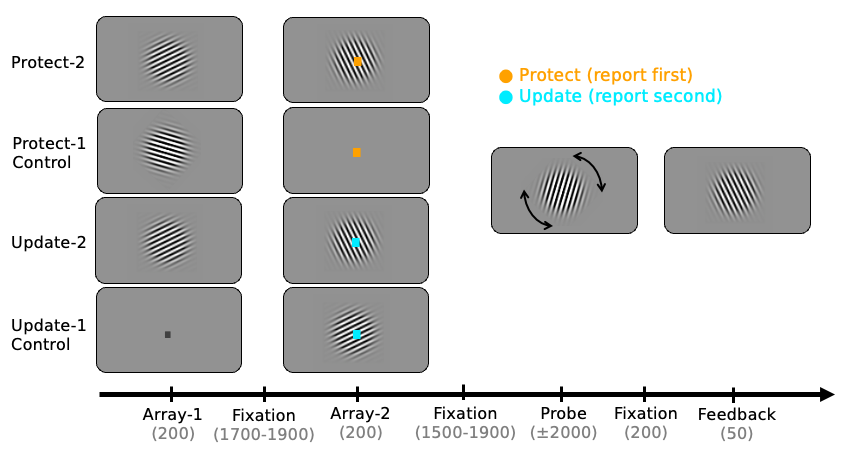
\includegraphics[width=0.9\textwidth]{figures/task_design.png} 
\caption[Experimental task design.]{Experimental task design. Participants were presented with two arrays that contained an oriented bar grating or a place holder fixation dot. On any given trial, either the first (25\% of trials), second (25\%), or both (50\%) orientations were presented. A colour cue that was presented on array 2 indicated the array that was relevant for the reporting stage later in the trial. The colour cue could indicate as relevant either the first array (“protect working memory content”) or the second array (“update working memory content”). On trials where only one orientation was presented the cue was redundant but presented. Note that the colour cue contingencies are displayed for visualisation purposes; mappings between colour and cue meaning were counterbalanced. After matching the orientation in the probe display to the orientation in memory, participants were presented with feedback in the form of a grating with the correct orientation. Timings in brackets are in milliseconds. Cue size in array-2 is enlarged for visualisation purposes.}
\label{fig:task_design}
\end{figure}


\subsection{Behavioural Analysis}
Response error was quantified by calculating the circular distance of the recalled orientation to the cued orientation. All responses were mapped onto a -180$^{\circ}$ to 180$^{\circ}$ space to compute circular error. In all between-trial analyses, we excluded the first trial of each block.\\


\subsection{Mixture Modelling}
To investigate the relative rate of responses to targets, guesses, and erroneous responses to the wrong target (‘swap errors’), we fit a classical mixture model frequently used in working memory literature \parencite{Schneegans2017, Bays2009, Zhang2008}. The model was fit separately for each condition (protect, 2 items; protect, 1-item control; update, 2 items; update, 1-item control). The mixture model estimated the precision of the von Mises distribution, target response rate, guess rate, and swap rate to the item that was presented on the same trial but not cued (only load-2 trials). The model provided single trial estimates of each of the three parameters. \\

\subsection{Performance Bias Calculation}
We calculated the performance bias (the circular difference between the response and the target orientation) as a function of the circular difference between the target orientation and the orientation that induced the bias (the previous target orientation on the preceding trial or the task-irrelevant grating on the same trial). We computed the difference between the target orientation and inducer through subtraction, with all angular differences mapped between -90$^{\circ}$ and 90$^{\circ}$. These distances were binned into 64 equally-sized bins. We computed the average signed error (bias) across all trials within each bin. To reduce noise, we applied a sliding window, computing the average response error over 25\% of the bins (16 bins). Edge artifacts were avoided by wrapping the angular differences around, to ensure the average was always computed over 16 bins. Subsequently, we sign-flipped the bias in bins with a negative distance and averaged over negative (-90$^{\circ}$ to 0$^{\circ}$) and positive distances (0$^{\circ}$ to 90$^{\circ}$) between target orientation and inducing orientation, resulting in 32 bins. The integral over absolute distances (0$^{\circ}$ to 90$^{\circ}$) calculated over the 32 bins for each condition and participant served as a measure of bias. \\

\subsection{MEG Acquisition}
Participants were seated in the MEG scanner after being instructed about the task specifics. They completed one practice block while seated in the scanner prior to MEG recording onset. Participants were instructed to maintain their gaze at the central fixation cross and to minimise blinking throughout the trial. 

Neuromagnetic data were acquired using a whole-head VectorView system including 204 planar gradiometers and 102 magnetometers (Elekta Neuromag Oy, Helsinki, Finland) in a magnetically shielded room. Throughout the experiment, participants’ head position was monitored continuously using index coils placed at four points on the head. Magnetic field strength was sampled at a rate of 1000 Hz and band-pass filtered on-line between 0.03 Hz and 300 Hz. In addition, vertical and horizontal electro-oculograms were measured using electrodes placed above, below, and adjacent to the eyes. Eye movements were monitored using an EyeLink 1000 (SR Research) eye tracker at a frequency of 1000 Hz.\\


\subsection{MEG Data Preprocessing} 
The data were pre-processed offline using Fieldtrip \parencite{Oostenveld2011}, OHBA software library (OSL) drawing on SPM8 (\url{http://www.fil.ion.ucl.ac.uk/spm}), and Elekta software. Prior to any preprocessing, the MEG data were visually inspected to remove and interpolate any sensors that displayed excessive levels of noise and were subsequently de-noised and motion corrected using Maxfilter Signal Space Separation \parencite{Taulu2004} before removing independent components related to cardiac and eye-blink artefacts. Data were epoched around the first grating and second grating (from 400 ms prior to grating onset to 900 ms after onset) and downsampled to 200 Hz. Trials with high variance in either gradiometers or magnetometers were identified and excluded using a generalised ESD \parencite[extreme studentised deviate;][]{Rosner1983} test at a 0.05 significance threshold. This resulted in 7.49\% ± 11.55\% (mean ± standard deviation) being excluded during preprocessing.  \\

\subsection{LDA Classification}
Data were further pre-processed, where magnitudes of magnetometers were approximately matched to gradiometers by multiplication (factor 20) and subjected to spatio-temporal decoding as described in \parencite{Hajonides2021, Wolff2017, Wolff2020}. Data from all 306 MEG sensors across a sliding window of 30 time points (150 ms) were concatenated into a vector. Pre-stimulus baselining was not applied to maintain stable information from previously presented stimuli. Dimensionality was reduced for each time point through a principal component analysis, maintaining 90\% of the variance (between 250 to 600 ms this was around 209 ± 39 components, mean ± std.). To train an LDA classifier, the data were split in train and test sets using 10-fold stratified cross-validation. Grating angles were binned into 10 equally spaced orientation bins (0$^{\circ}$ to 18$^{\circ}$, 18$^{\circ}$ to 36$^{\circ}$, 36$^{\circ}$ degree to 126$^{\circ}$, 126$^{\circ}$ to  144$^{\circ}$, 144$^{\circ}$ to 162$^{\circ}$, 162$^{\circ}$ to 180$^{\circ}$). For each trial and time point, we thus obtained 10 LDA distances estimating the likelihood for each of the bins. Tuning curves were constructed by aligning evidence across trials around the same category bin. In cross-decoding analyses, LDA classifiers were trained on orientation bins of one event (e.g., presented grating) but classifier evidence aligned around bins of another orientation (e.g., target orientation on the previous trial). The resulting tuning curves were convolved with a cosine.\\

\subsection{Bias Computation}
For within-trial biases, we assessed processing of the second grating and only considered load-2 trials. The classifier was trained on all presentations of the second grating and bin likelihoods were generated for each trial. For between-trial analyses, we analysed orientation processing of both the first and second grating. For this reason, we trained the classifier on all trials and generated bin predictions for all trials. 

Subsequently, based on the results from the performance-bias analyses, we selected trials where the angular distance between the inducer and the grating orientation on the display led to a significant behavioural bias at the group level. In the case of the within-trial repulsive bias, the inducer was the orientation of the first grating on the same trial; for the between-trial analyses the inducer was the target orientation on the previous trial. As a dependent variable, we considered likelihood estimations for each orientation bin, where we expect the highest likelihood for the angular bin that has zero offset to the presented orientation and decreasing likelihoods for bins with larger angular distances to the presented orientation. We separately assessed likelihood estimations on trials where the inducer orientation was clockwise (CW) or counterclockwise (CCW) with respect to the current orientation. For both CW and CCW trials we separately averaged the evidence from the orientation bins CW (-72$^{\circ}$ to -18$^{\circ}$) and evidence from the CCW bins (18$^{\circ}$ to 72$^{\circ}$). Symmetry scores were computed by obtaining the difference between the two groups of angular bins (CW minus CCW). Finally, we calculated an overall neural bias score by subtracting symmetry scores on trials with CW vs. CCW inducers. Attractive biases resulted in a positive score (i.e., trials with CW angular distances resulted in more CW evidence, CCW angular distances resulted in more CCW evidence), whereas repulsive biases resulted in a negative score (i.e., CW angular distances resulted in more less CW evidence than CCW trials, and vice versa). 

\subsection{Statistical Testing}
Statistical tests were computed using both JASP \parencite{JASP2020} and Scipy \parencite{Virtanen2020}. 

We tested the time series of cosine-convolved classifier evidence against zero using a cluster-based permutation test \parencite[using MNE; ][]{Gramfort2013}. We ran 100,000 iterations and a F-statistic threshold of 2.093 (p < .05 with 19 degrees of freedom). The clusters where groups of time points were significantly different from zero are indicated in the relevant figures using horizontal lines. Cluster-based permutation testing was also applied to performance bias across angular distance between the presented orientation and the inducer orientation.


Estimating the shifts in the tuning curves relied on the presence of a tuning curve. Hence, we only used the average of all timepoints where cosine-convolved classifier evidence for the presented grating orientation was significantly above zero in our comparison analyses (in all reported time averages, time points between 250 and 600 ms were used). 

All tests were two-sided unless stated otherwise. 


\section{Results}
\subsection{Error Rates}
%



Participants were accurate in reproducing the target orientation (mean response error 11.73$^{\circ}$ ± 0.70$^{\circ}$ SEM; mean standard deviation 17.61$^{\circ}$ ± 1.07$^{\circ}$ S.E.M., see Table 1 for condition-wise performance). A 2-by-2 repeated-measures ANOVA showed main effects of cue type $(F\textsubscript{1,19} = 16.49, p < .001, \eta\textsuperscript{2} = 0.374)$ and stimulus load $(F\textsubscript{1,19} = 29.78, p < .001, \eta\textsuperscript{2} = 0.075)$. 
Cue type was significant for both load conditions, with absolute error higher on protect (1-item control) trials than on update $(\text{1-item control; Table ~\ref{tab:error_rates}; }t\textsubscript{19} = 3.948, \text{Bonferroni-corrected }  p < .001, d = 0.883)$ and higher on protect (2 items) than on update (2 items) trials $(t\textsubscript{19} = 3.972, p < .001, d = 0.888)$. By contrast, load primarily affected the protect conditions. Error was higher on protect (2 items) than on protect (1-item control) trials $(t\textsubscript{19} = 5.665; p < .001, d = 1.267)$ but did not significantly differ between update (2 items) and update (1-item control) trials $(t\textsubscript{19} = 1.885, p = .075, d = 0.421)$, leading to a significant interaction between the two factors $(F\textsubscript{1,19} = 10.90, p = .004, \eta\textsuperscript{2} = 0.026)$. Control analyses using mixture modelling confirmed that errors originated predominantly from varying precision in responses to the orientation of the correct target grating (\textbf{Supplementary information}).
%

  
\bigskip

\begin{table}[htpb]

\begin{center}
\caption{\textbf{Descriptive statistics of error for all experimental conditions.}}

\begin{tabular}{cccc}

\toprule
& \textbf{Protect} & \textbf{Update} \\
\midrule
1 item & 11.91$^{\circ}$ (±4.61$^{\circ}$) & 8.96$^{\circ}$ (±2.52$^{\circ}$)  \\
2 items & 14.69$^{\circ}$ (±5.38$^{\circ}$) & 9.79$^{\circ}$ (±2.89$^{\circ}$)  \\
\bottomrule
\end{tabular}
\end{center}


\begin{center}
\small\textit{Note}. \fontsize{10}{12}\selectfont Mean Absolute Error (± Std. Dev.). All units are in degrees.
\end{center}
\label{table:error_rates}
\end{table}

\subsection{Performance biases within trials}
We analysed within-trial biases in behavioural performance by assessing whether the reported orientation was systematically reported as closer to or further away from the non-target orientation on the same trial. \textbf{Figure ~\ref{fig:behav_repulsive}A} shows the performance bias for all absolute angular distances between the first and second grating orientation for update and protect trials. After encoding the first grating, participants either protected their memory content from interference of the second grating or updated their working memory to represent the second grating orientation. On trials with protect cues, there was no significant bias towards or away from the interfering second grating orientation that was not relevant to the task at hand $(t\textsubscript{19} = 0.74, p = .467)$. In contrast, trials with update cues revealed significant biases away from the initially encoded first grating orientation $(t\textsubscript{19 }= -2.33, p = .031; \text{illustrated in \textbf{Figure ~\ref{fig:behav_repulsive}B}})$. The repulsive bias on update trials was confirmed using a cluster-based permutation test, showing a significant (cluster-corrected p < 0.05) cluster when the angular distance between the two orientations was between 8$^{\circ}$ and 48$^{\circ}$ (\textbf{Figure ~\ref{fig:behav_repulsive}A}). Note that we did not consider load-1 control trials for this within-trial bias analysis, as these trials only contained a single item. \\

\begin{figure}
\centering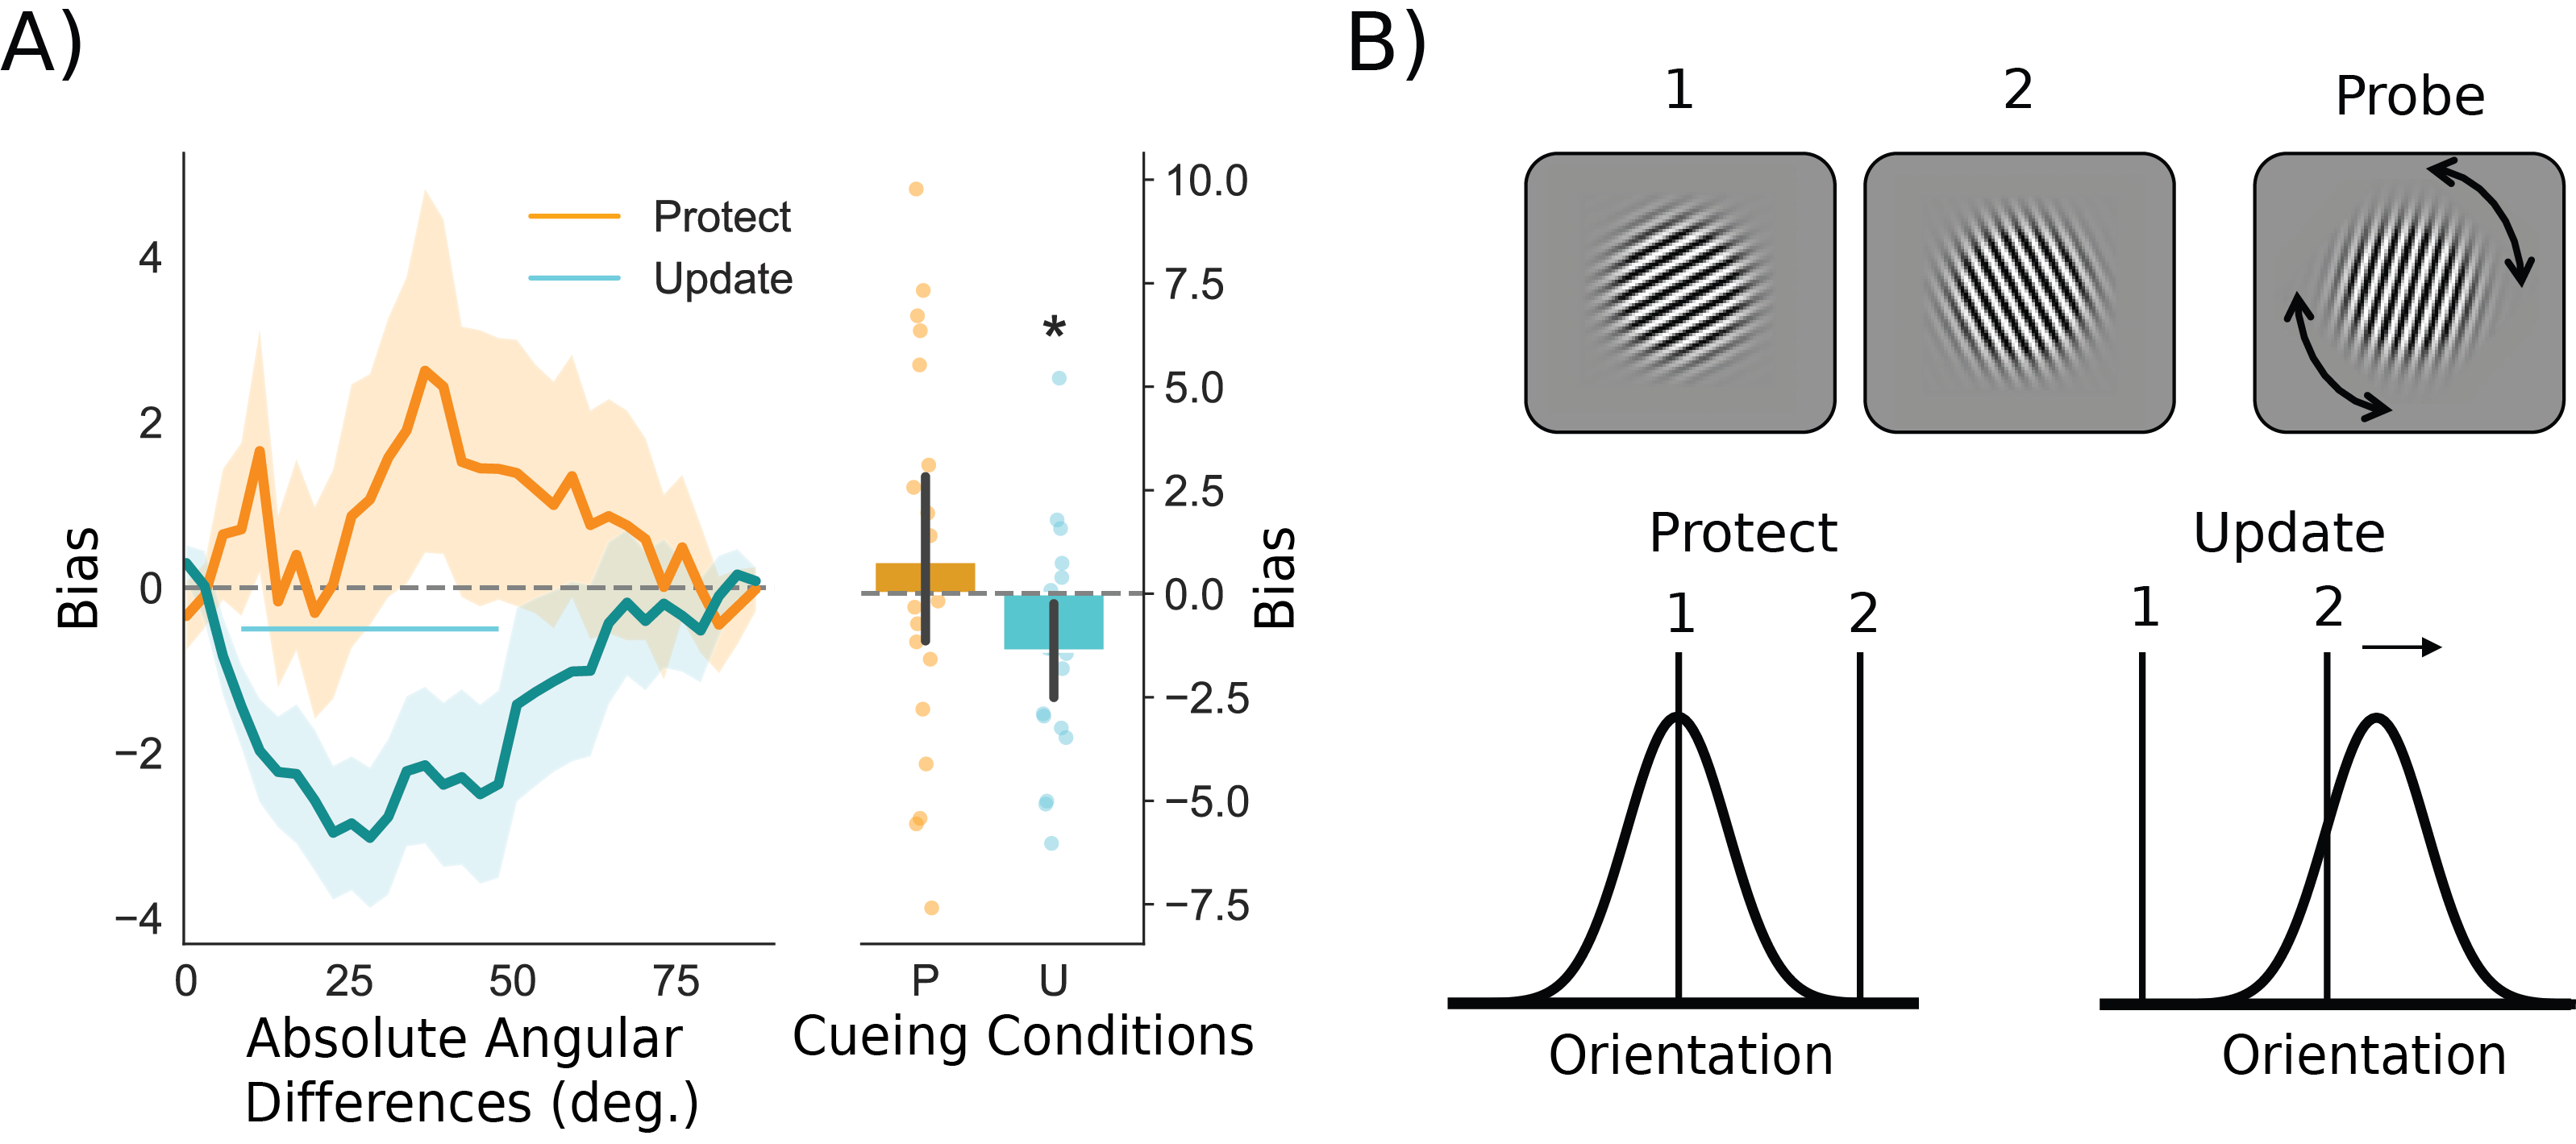
\includegraphics[width=0.9\textwidth]{figures/figure2_behav_within_trial.png} 
\caption[Within-trial repulsive performance biases.]{Within-trial repulsive performance biases. A) Within-trial bias as a function of the absolute angular distance between the two presented orientations. Trials were split for protect and update cues on load-2 trials. Shading indicates standard error of the mean. The horizontal line indicates a cluster of significant performance biases for a range of angular difference. The right panel shows the sum of integrals per subject. Error bars show 95\% confidence intervals. P = protect trial; U = update trial. B) Schematic of the within-trial performance bias. A repulsive performance bias is observed for update trials only.}
\label{fig:behav_repulsive}\end{figure}

\subsection{Attractive Performance Bias Between Trials}
We next evaluated the between-trial bias on responses of the current trial towards the orientation that was cued on the previous trial (\textbf{Figure ~\ref{fig:behav_attractive}}). Again, we assessed the performance bias as a function of angular differences between the target grating on the current and on the previous trial. The analysis also considered the position of the target grating on the current trial (1\textsuperscript{st} or 2\textsuperscript{nd}) and the stimulus load on the current trial (load 1 or 2). For consistency, we term all trials where participants report the first grating orientation \textit{protect trials} and trials where participants report the second orientation \textit{update trials}, regardless of the number of gratings presented. Again, we quantified the integral of the bias across angular distances between targets on the current and previous trial \textbf{Figure ~\ref{fig:behav_attractive}A, B}. In contrast to the repulsive bias described in the previous section, here we found that all conditions showed an attractive performance bias (all p < .05 in two-sided statistical tests; illustrated in \textbf{Figure ~\ref{fig:behav_attractive}E}). The attractive serial bias was most pronounced for small to intermediate angular distances between the inducer and current orientation (0 - 60$^{\circ}$, see also \textbf{Supplementary Results}). A repeated-measures ANOVA on the integrals indicated an effect of cue type, with larger biases occurring in protect trials $(F\textsubscript{1,19}  = 5.706, p = .027, \eta\textsuperscript{2} = .172)$, but not of the number of gratings presented in a trial $(F\textsubscript{1,19}  = .980, p = .335, \eta\textsuperscript{2} = .007)$. The two factors did not interact $(F\textsubscript{1,19}  = .377, p = .547, \eta\textsuperscript{2} = .002)$. This shows that it is not the updating or protecting perse that matters for this bias, but rather the time from encoding of the relevant item on the current trial, since the previous trial.


\begin{figure}
\centering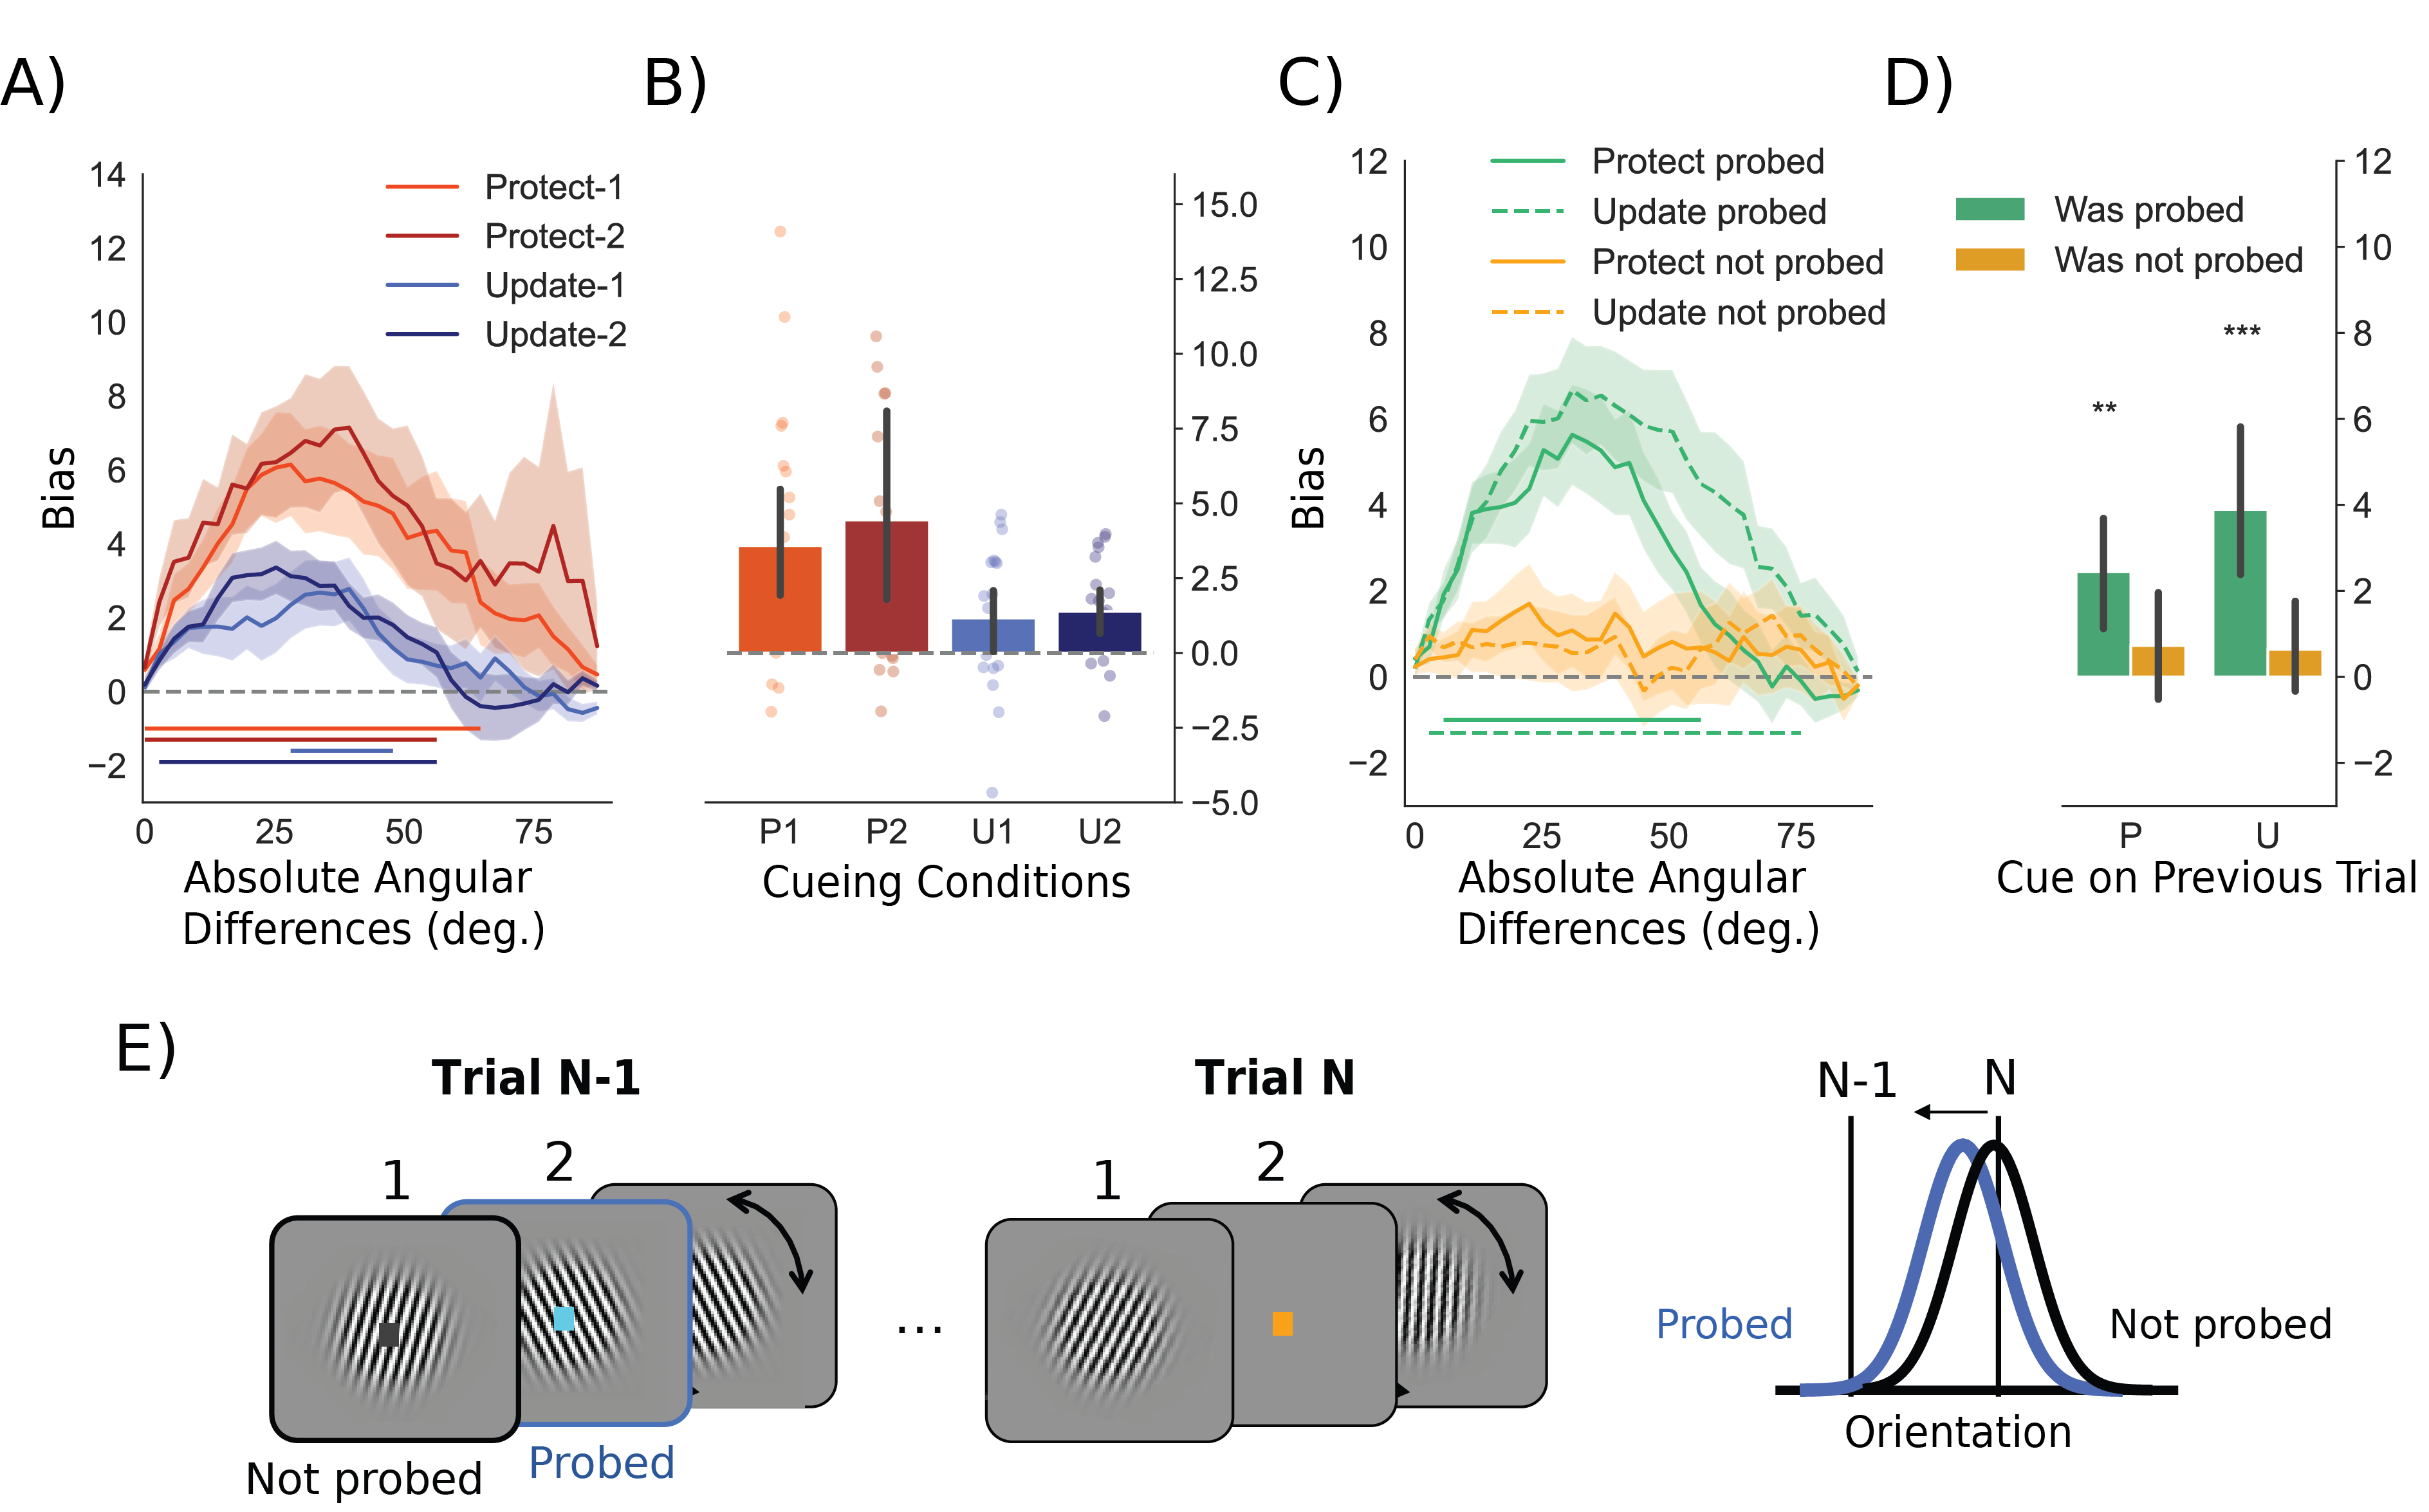
\includegraphics[width=0.9\textwidth]{figures/figure3_behav_between_trial.png} 
\caption[Attractive behavioural biases towards the relevant target orientation on the previous trial.]{Attractive behavioural biases towards the relevant target orientation on the previous trial. A) Line plots for the attractive between-trial bias as a function of the absolute angular distance between the target orientation on the previous trial and the presented grating. Shading indicates standard error of the mean. Horizontal lines indicate clusters of significant performance biases for a range of angular difference. B) Bar plots indicate the average sum of integrals per subject and per condition as seen in panel ~\ref{fig:behav_attractive}A. C) Line plots show the attractive between-trial bias as a function of the absolute angular distance between the probed angle on the previous trial (green) or the presented but not probed angle in the previous trial (orange). The horizontal lines indicate cluster-corrected angular distances for which the bias is significant. D) Integrals of the response data shown in panel ~\ref{fig:behav_attractive}C where positive values indicate an attractive bias. P = Protect cue on previous trial; U = Update cue on previous trial. E) Schematic illustrating the attractive behavioural performance bias between trials. Behavioural responses on trial N were biased towards the orientation that was tested for recall (depicted in blue) and not towards the orientation that was not tested (black) on trial N-1. All error bars indicate 95\% confidence intervals.}
\label{fig:behav_attractive}\end{figure}


\subsection{Task Dependence of Attractive Performance Bias Between Trials}
Next, we repeated the same between-trial analyses but investigated the role of task relevance and cue type on the previous trial. This allowed us to test for and compare behavioural biases elicited by the probed (and reported) orientation and by the unreported orientation on the previous trial. We also tested whether the cue type on the previous trial affected bias on the current trial. We only looked at trials in which two orientations were presented on the previous trial.


A repeated-measures ANOVA on the integral of the performance bias for task relevance and cue type confirmed an effect of task relevance $(F\textsubscript{1,19}  = 14.684, p = .001; \text{\textbf{Figure ~\ref{fig:behav_attractive}D}})$ but showed no effect of cue type $(F\textsubscript{1,19}  = 1.423, p = .248)$ or interaction $(F\textsubscript{1,19} = 1.633, p = .216)$. Task-relevant orientations in trials of either cue type led to a significant bias $(\text{previous trial protect (2 items): } t\textsubscript{19} = 3.524, p = .002; \text{previous trial update (2 items): } t\textsubscript{19} = 4.476, p < .001)$. Unprobed orientations did not lead to a significant bias $(\text{both } p > .2)$. No reliable difference was observed between the strength of the bias between update (2 items) or protect (2 items) conditions on previous trials $(t\textsubscript{19} = 1.691, p = .107)$. Following up, we assessed the performance bias as a function of the angular distance between the current target orientation and previously presented orientations. Cluster-based permutation testing showed an attractive bias towards the task-relevant orientation on the previous trial when a protect cue $(p = .001; 6^\circ \text{ – } 56^\circ; \text{\textbf{Figure ~\ref{fig:behav_attractive}C}})$ or an update cue $(p < .001; 3^\circ \text{ – } 76^\circ)$ was presented on the previous trial. For unreported orientations no bias was observed (no candidate clusters for protect or update cue). Together, this pattern of results is summarised in \textbf{Figure ~\ref{fig:behav_attractive}E}, showing an attractive between-trial bias, but only with regard to items that were relevant in the previous trial. \\


\subsection{Neural Classification of Presented Orientations}
We extracted data from all 306 sensors ranging from 400 ms prior to stimulus onset up to 900 ms post stimulus onset. LDA classification reflected significant evidence for the presented orientation after visual onset of the grating \textbf{Figure ~\ref{fig:decoding}}. This revealed both significant decoding of the first grating orientation $(100 \text{ – } 615 \text{ms}; p < .001)$ as well as the second grating orientation $(95 \text{ – } 590 \text{ms}; p < .001)$. A non-significant trend was observed for the evidence of the first grating orientation following the presentation of the second grating $(250 \text{ – } 600 \text{ms}; t\textsubscript{19} = 1.971; p = .063; \text{see also cross-decoding analyses below})$. There was no difference in classifier evidence after an update or protect cue $(250 \text{ – } 600 \text{ms}; t\textsubscript{19} = 0.798; p = .435)$. \\


\begin{figure}
\centering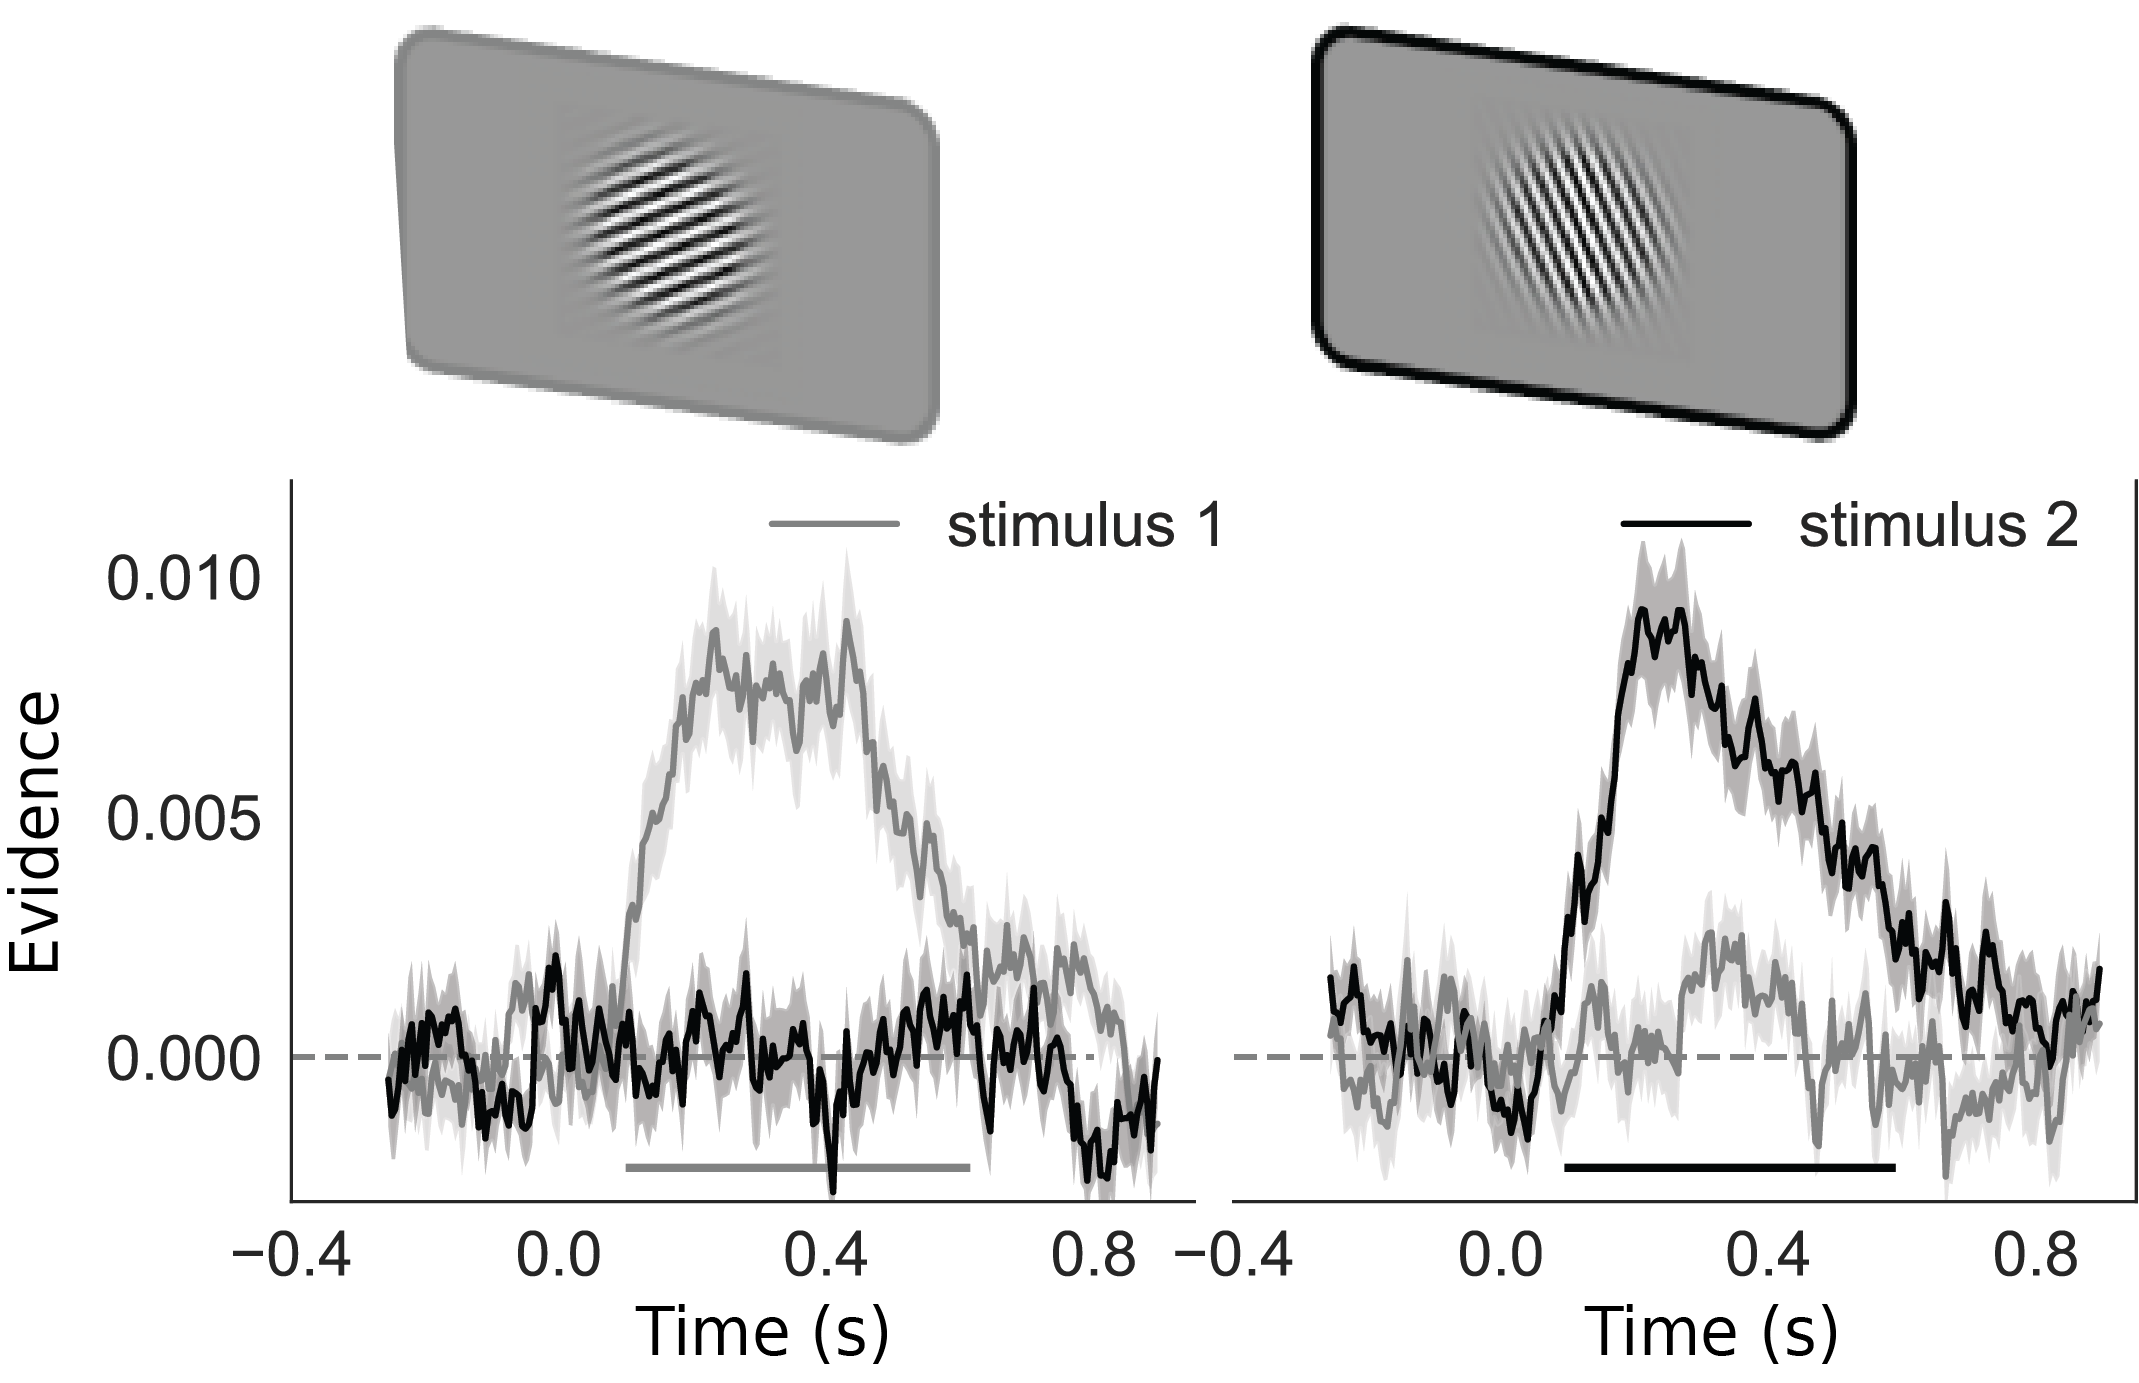
\includegraphics[width=0.7\textwidth]{figures/figure4_decoding} 
\caption[Orientation decoding of presented grating.]{Orientation decoding of presented grating. Training an independent classifier to decode the first or second grating orientation in either the first- or second-time interval. The cue in the second display is removed for visualisation purposes. Error bars indicate standard error of the mean. Horizontal lines indicate periods of significant grating orientation decoding after cluster-based permutation tests against zero, p = .05.}
\label{fig:decoding}\end{figure}


\subsection{Within-trial Classification Bias Away From Previous Stimulus}
To investigate how information from the second grating was modulated by information from the first grating, we separately assessed trials with protect and update cues. Doing so, we evaluated the LDA evidence tuning curves elicited by the second grating. For these analyses we again only selected trials where both gratings were presented. We separated trials where the first grating was clockwise vs. counterclockwise relative to the second grating (angular distance of 10$^{\circ}$ - 50$^{\circ}$, based on behavioural results, see \textbf{Figure ~\ref{fig:behav_repulsive}A, B}). We considered the average of time points between 250 – 600 ms for all future analyses, since in this time window stimulus orientation could be decoded with reliable accuracy (see \textbf{Figure ~\ref{fig:decoding}} and grey-shaded area in \textbf{Figure ~\ref{fig:within_decoding}}). Echoing the performance biases, no significant bias occurred on protect trials $(\text{\textbf{Figure ~\ref{fig:within_decoding}A, B}};  t\textsubscript{19} = -0.723; p = .478)$. However, on update trials, we observed a repulsive effect, away from the previously encoded grating orientation $(\text{\textbf{Figure ~\ref{fig:within_decoding}C, D}}; t\textsubscript{19}  = -3.52; p = .002)$. 

Notably, there was no correlation, across participants, between the magnitude of the bias in the behavioural and neural data on protect trials $(r = .010; p = .968)$ or update trials $(r = -.328; p = .158)$.\\


\begin{figure}
\centering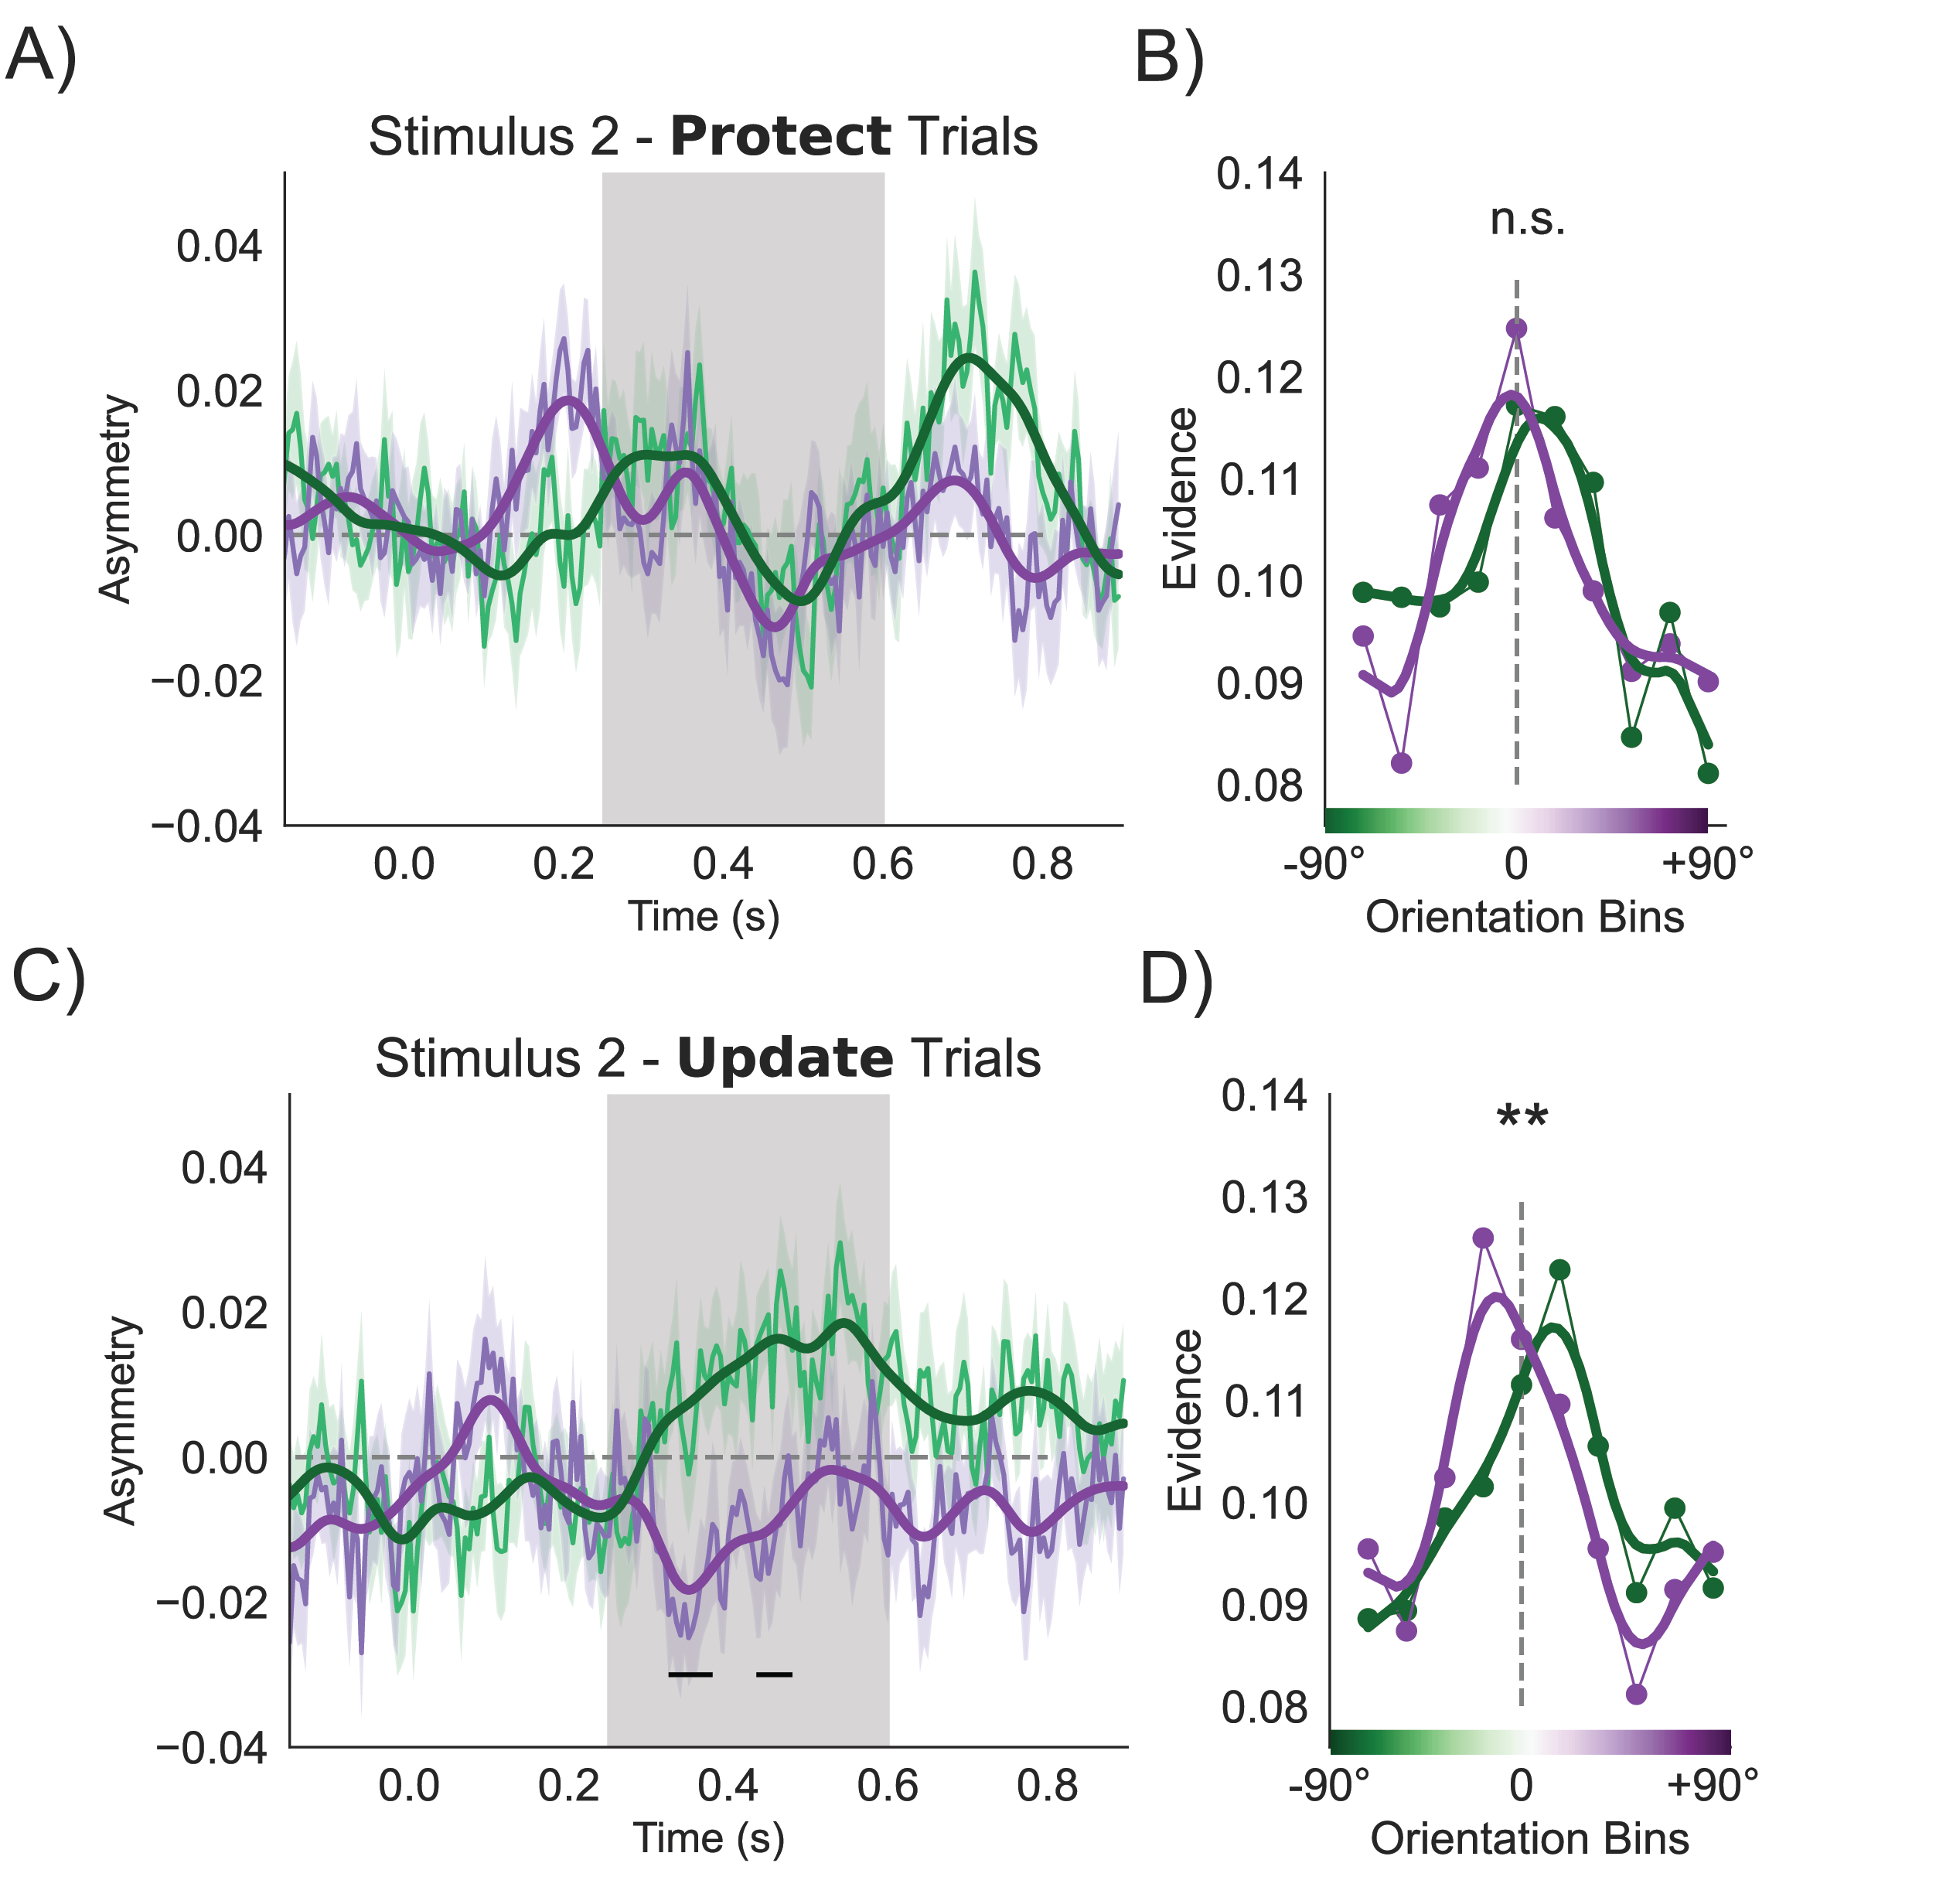
\includegraphics[width=0.7\textwidth]{figures/figure5_within_trial_decoding} 
\caption[Shift in tuning curve relative to previous grating orientation. ]{Shift in tuning curve relative to previous grating orientation. A) Asymmetry scores following the presentation of the second grating on protect (2 items) trials. The first grating orientation had a CCW (purple) or CW (green) angular distance relative to the current grating orientation. The shaded area indicates the time interval (250 - 600 ms) used for statistical analysis and to generate the tuning curves in the right panel. Smoothing (thicker lines in darker colours) was applied for visualisation purposes. B) shows the tuning curves with evidence for the presented grating orientation for trials with CW or CCW angular distances relative to the first rating. For visualisation purposes, data points were interpolated (from 10 to 50 data points) and fitted using a Savitzky-Golay filter (with a window length of 9 data points and polynomial of order 1). C) Asymmetry scores for update (2 items) trials, where participants encoded the grating orientation on screen into working memory with a bias away from the grating orientation that was presented earlier on the same trial. Shading indicates standard error of the mean. D) shows data from the grey-shaded region in panel ~\ref{fig:within_decoding}C. Horizontal lines indicate periods of significant bias on unsmoothed data after cluster-based permutation tests against p = .05. }
\label{fig:within_decoding}\end{figure}

\subsection{Repulsive Neural Biases Between Trials Away From Sensory History}

To probe for neural between-trial biases, we used the same approach as for within-trial neural biases. We tested the LDA-evidence derived during the stimulus encoding period for systematic deviations in likelihood estimations as a function of the angular distance between the current orientation and the probed orientation on the previous trial. If the behavioural between-trial bias reflects neural modulation during encoding of sensory features, we would expect to see an increase in likelihood estimations for orientations presented on the previous trial in line with the attractive performance bias. We trained the classifier on data following presentation of both the first and second grating orientation combined and included all cue types and loads. Informed by our behavioural analyses on between-trial performance biases, for the test set we selected trials where the previous probe angle had a relative difference of 0$^{\circ}$ – 60$^{\circ}$ (\textbf{Figure ~\ref{fig:behav_repulsive}C, D}; derived from significant angular differences) CW or CCW from the presented grating orientation. The results were qualitatively the same and remained significant when other angular ranges were selected. 

Contrary to our expectations, classifier evidence was significantly shifted away from the target orientation on the previous trial $(\text{250 – 600 ms post grating onset; } t\textsubscript{19} = -2.83, p = .011; \text{\textbf{Figure ~\ref{fig:between_decoding}A, B}})$ rather than mirroring the attractive behavioural bias. In practice, this would mean that the cued orientation on the previous trial was CW, classifier evidence for CCW bins was increased, and vice versa. The repulsive bias away from the target on the previous trial trended towards significance for the first $(t\textsubscript{19} = -1.78, p = .090)$ and was significant for the second grating $(t\textsubscript{19} = -2.43, p = .025)$ in the current trial when considered separately (\textbf{Figure ~\ref{fig:between_decoding}C}). The between-trial repulsive bias during stimulus-two processing was present if no orientation was presented in the first interval $(t\textsubscript{19} = -2.69, p = .014)$ but not when the first grating was also presented $(t\textsubscript{19} = -1.68, p = .110)$. 

Next, we tested whether this repulsive neural bias was affected by the task relevance of the grating and by the cueing condition of the previous trial. We quantified the bias for task-relevant and task-irrelevant grating orientations on the previous trial. Only trials where the previous trial was load-2 were included in this analysis. When averaging the neural bias over 250 – 600 ms, the task-relevant orientation showed a repulsive neural bias (t\textsubscript{19} = -2.78, p = .012), but we found no neural bias for task-irrelevant orientations $(t\textsubscript{19} = -0.33, p = .743)$, though this difference did not reach significance $(t\textsubscript{19} = 1.80, p = .088)$. Yet, cluster-based permutation testing indicated a significant cluster where task-relevant orientations had a significantly stronger repulsive bias than task-irrelevant orientations $(500 \text{ – } 550 \text{ms}; p = .039)$. \\

\begin{figure}
\centering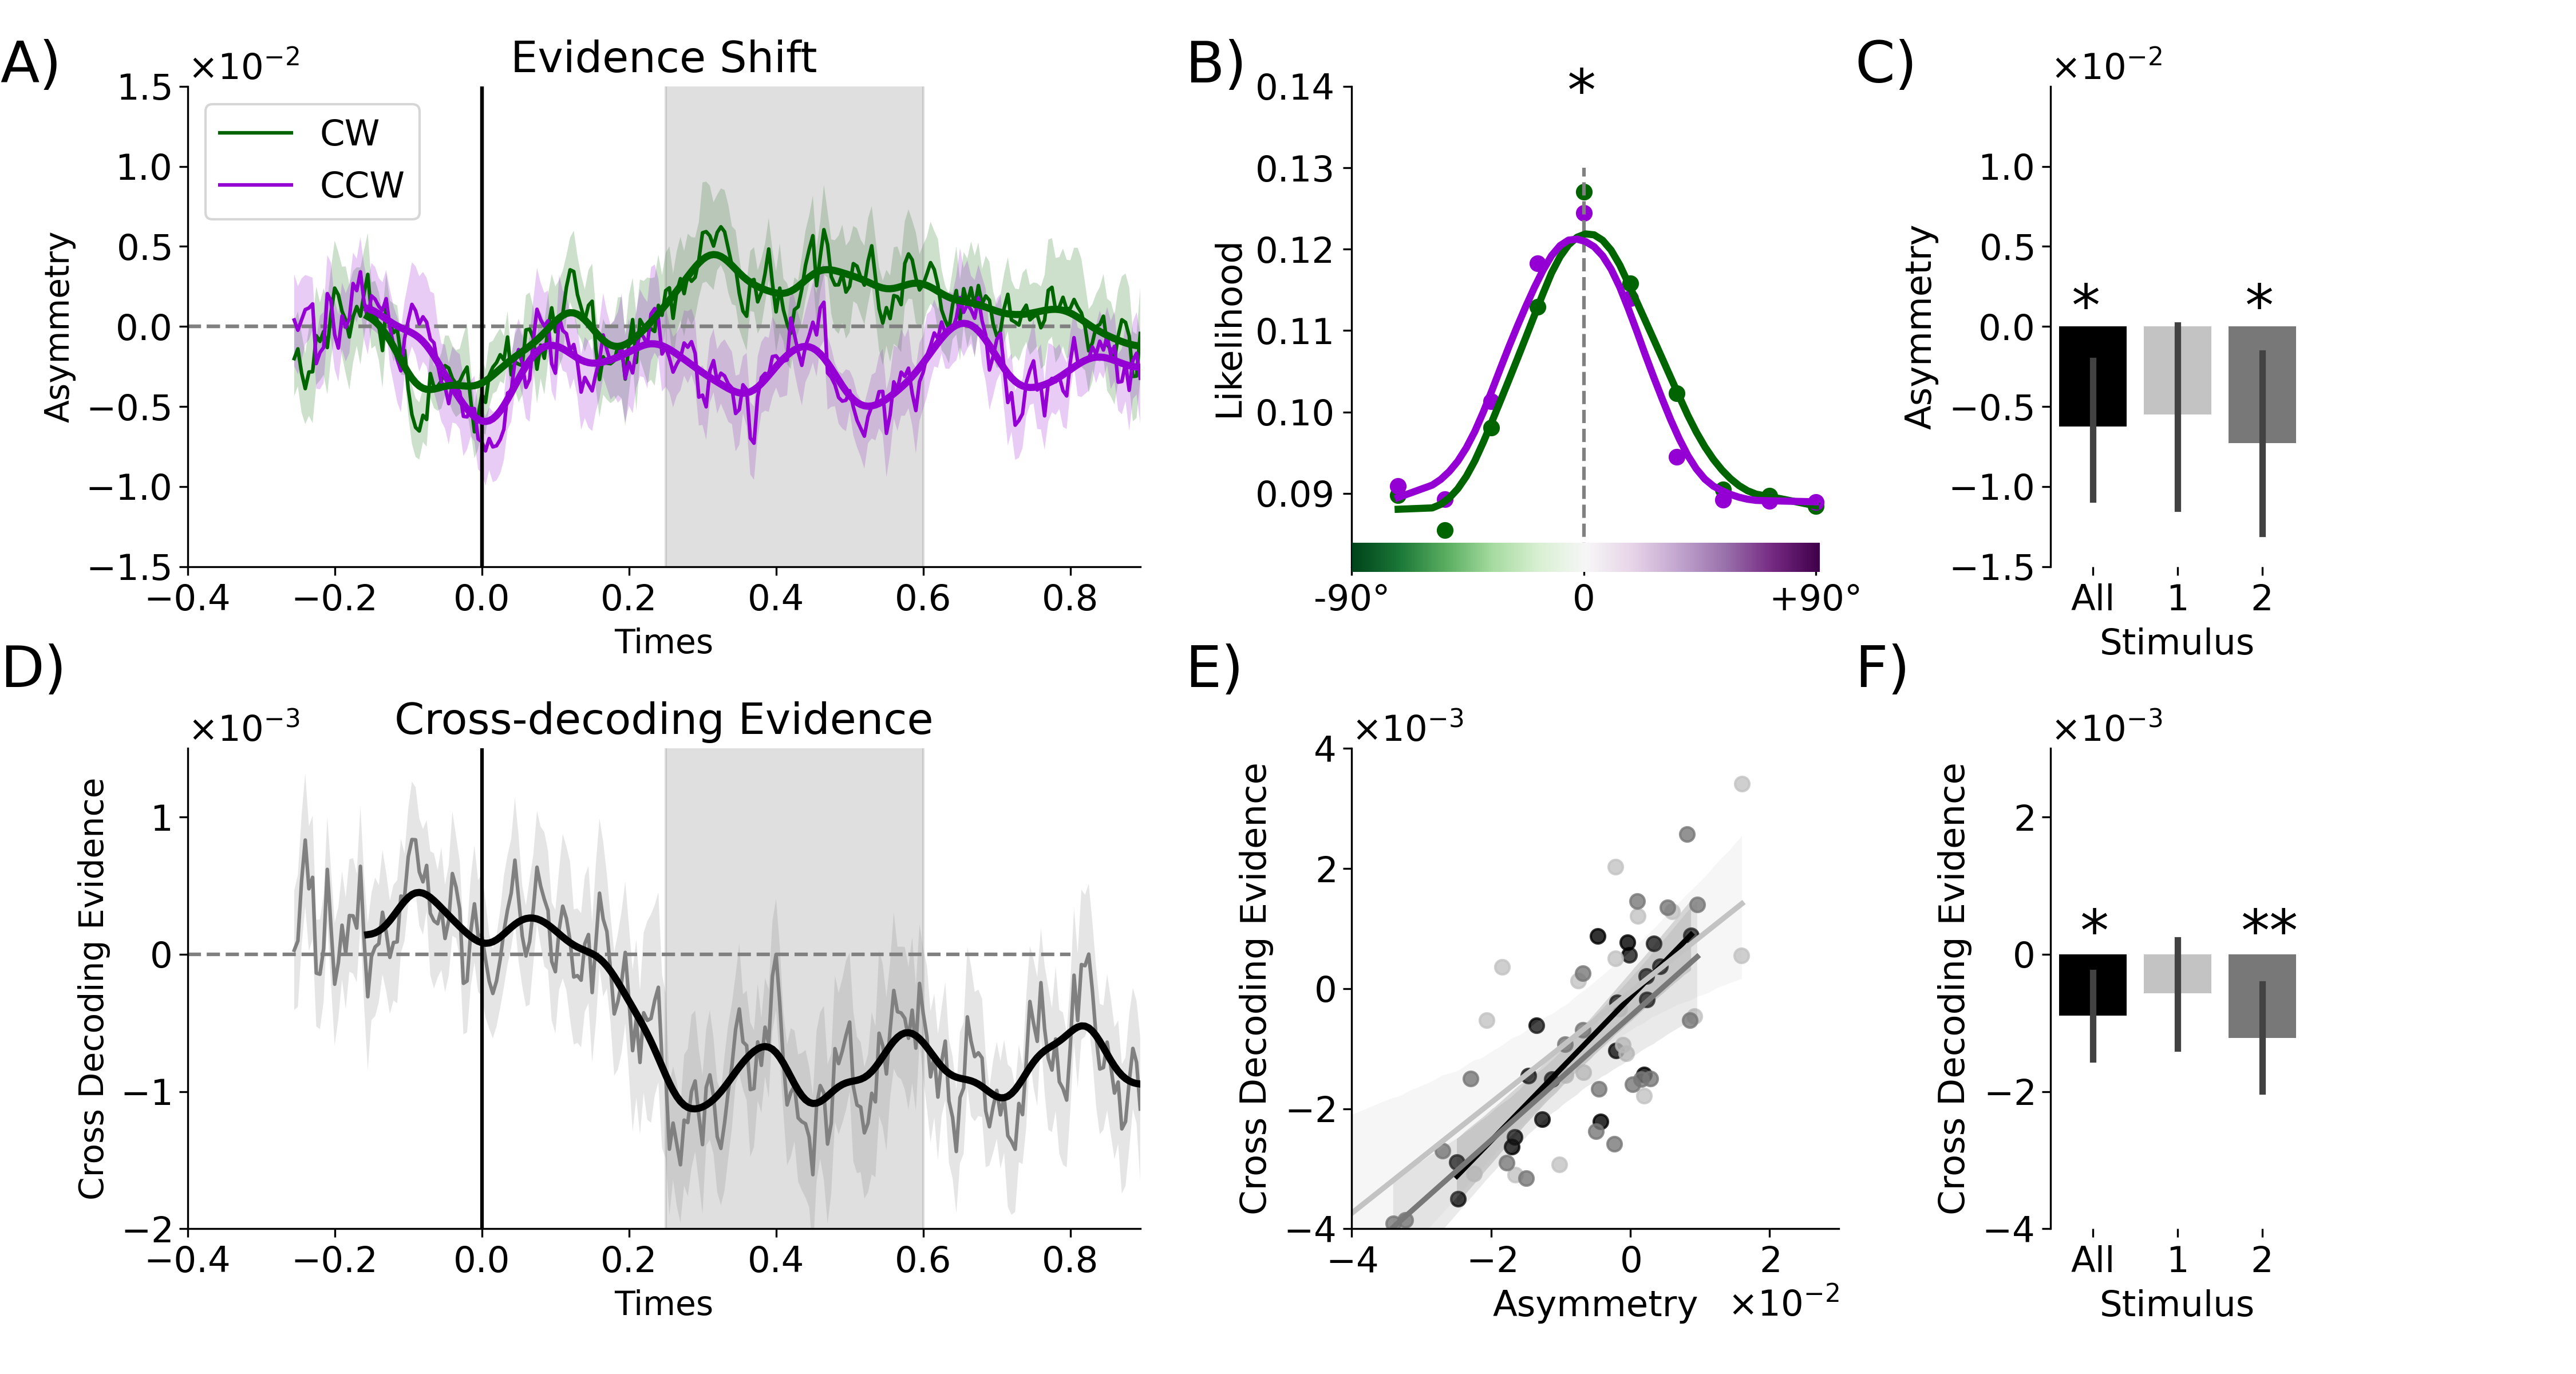
\includegraphics[width=0.9\textwidth]{figures/figure6_between_trial_decoding} 
\caption[Bias on encoding imposed by previous trial.]{Bias on encoding imposed by previous trial. A) Asymmetry index for trials with a CW or CCW angular distance (0$^{\circ}$ – 60$^{\circ}$) between the cued item on the previous trial and the presented grating (collapsed across the first and second grating). Asymmetry index time course is shown relative to the onset of grating presentation. A one-dimensional Gaussian filter with a kernel of 15 ms was applied to the data for visualisation purposes. The grey shaded area indicates which time points (250-600 ms) are used for analyses described in text and in panels ~\ref{fig:between_decoding}B, C, and E. B) Average LDA orientation-likelihoods for trials with CW (green) and CCW (purple) angular distances with respect to the previous trial. Evidence is lower for CW orientation bins when in the previous trial a CW orientation was cued, and vice versa for CCW orientations. The same interpolation was applied as described in Figure Figure ~\ref{fig:within_decoding}. C) Average bias relative to the previously cued orientation across all stimuli and for the first and second orientation separately. D) Cross-decoding evidence for the previously cued orientation (classifier trained on current orientation), locked to grating presentation. Same conventions as in panel A. E) Correlations between asymmetry index panel ~\ref{fig:between_decoding}A and cross-decoding evidence from panel D for grating orientation processing of all stimuli combined (black), first grating (light grey) and second grating (dark grey). A least-squares linear regression model was applied for each of the conditions, with shaded 95\% confidence intervals estimated using bootstrapping. F) Cross-decoding evidence from panel ~\ref{fig:between_decoding}D summarised for all stimuli and separately for the first and second grating, with 95\% confidence intervals. *: p < .05, **: p < .01}
\label{fig:between_decoding}\end{figure}

\subsection{Cross-Decoding Evidence for Previously Presented Stimuli}

If information about the previously presented orientation is still partially present in the visual system during and after the presentation of the current grating orientation, it could interact with encoding. One possibility is that the lingering representation is in an orthogonal representational format, which is different from sensory coding of features \parencite{Libby2021}. This means that there is little to no overlap between the activation pattern elicited during sensory input and the pattern related to the lingering representation of that same grating orientation. A classifier trained to separate perceptual information would not cross-generalise if tested on the memory code if this code is orthogonal. Alternatively, the lingering code could be present in a stable representation that shares similarity with incoming sensory information. If this were the case, the classifier, trained on the data from the second grating orientation, would cross-generalise and identify information about the first grating.

We adapted cross-decoding to detect lingering orientation-selective activity from the previous trial \parencite[also see ][]{Wan2020}. After training the classifier for the presented orientation and testing for evidence of the previous trial’s target orientation, we observed significant negative classifier evidence in the period of 250 – 600 after grating onset $(\text{\textbf{Figure ~\ref{fig:between_decoding}F}; concatenating over grating one and grating two: }t\textsubscript{19} = -2.820, p = .011\text{; grating one alone, }t\textsubscript{19} = -1.376, p = .185\text{; grating two, }t\textsubscript{19} = -2.951, p = .008)$.

Negative classifier evidence indicates that, while information is still present about the previous orientation, orientation-selective patterns may be sign-reversed relative to stimulus encoding. This suppression of evidence for the previous trial’s orientation could have been the cause of the apparent repulsive bias in the decoding of the current trial’s orientation. If this was the case, we would expect the two measures to be negatively correlated: stronger suppression of the previous orientation (negative classifier evidence) should lead to a stronger repulsive bias for the current orientation. We tested whether the magnitude of the between-trial neural bias and cross-decoding of previous trial were significantly correlated using Pearson correlations across participants. We found a significant correlation when assessing all grating presentations together $(\textbf{Figure ~\ref{fig:between_decoding}E}; r = .832, p < .001\text{; grating one, }r = .685, p < .001\text{; grating two, }r = .751, p < .001)$. 

No correlation was observed between the attractive behavioural performance bias and the magnitude of the repulsive shift in the neural data $(r = .186, p = .432)$ nor with the magnitude of negative decoding $(r = .144, p = .544)$.

The cross-decoding analysis and the correlation between cross-decoding and repulsive bias were repeated for the within-trial analyses in the previous section (see \textbf{Supplementary Figure 1}. These results conceptually confirmed the results reported here, although not all analyses reached significance. 


\section{Discussion}
The present study investigated biases from previously perceived and memorised information on neural coding and behavioural responses. We observed both neural and behavioural biases that demonstrate interactions between past and present sensory processing. Orientations presented on the same trial exerted repulsive biases on currently perceived orientations. In contrast, task-relevant orientations on the previous trial exerted an opposite, attractive bias, altogether providing evidence for two counteracting biasing processes. Multivariate decoding of neural data indicated that the two types of performance biases may arise from modulations acting on different stages of stimulus processing. Repulsive biases reflect at least in part modulation of sensory processing during item encoding, possibly reflecting mechanisms akin to visual adaptation that could promote visual discriminability. In contrast, the attractive performance bias observed across trials had no equivalent modulation at the sensory level. Interestingly, a neural repulsion occurred instead, suggesting the operation of post-perceptual modulatory mechanisms that can override any early sensory modulation and lead to attractive performance biases.


The present behavioural results provide evidence of two types of performance bias. Firstly, We identified a repulsive performance bias away from the first orientation in a trial. This bias was observed after participants updated their working-memory content to represent a second orientation. There was no retrospective repulsive bias when participants ignored the second grating and reported the first orientation, even though the second grating was presented closer in time to the probe. Secondly, participants’ responses on the current trial were biased towards task-relevant orientations on the previous trial \parencite[c.f., ][]{Bae2020, Fischer2020}. The attractive bias appeared strongest for items that were presented closest in time to the previous trial (first grating presentation) but was also present for the second grating, albeit with a smaller magnitude. Together, these results confirm a repulsive within-trial and an attractive between-trial performance bias.

Previously perceived stimuli generated a repulsive shift in orientation decoding, observed shortly after onset of grating presentation. This repulsive bias was only present when the presented orientation was task-relevant and therefore encoded into working memory. By contrast, task-irrelevant gratings that were not encoded into working memory could be decoded with similar precision, but did not exhibit a significant bias. Gratings from previous trials that were associated with an attractive performance bias also led to repulsive neural biases during working memory encoding. Only task-relevant orientations led to a repulsive bias. These results suggest a consistent bias that is carried forward from previous sensory processing. This repulsive bias may arise from sensory adaptation, but in the present study appears not to be a completely automatic process. Instead, the modulation by task-relevance suggests the bias is context-dependent. 

Visual adaptation has been proposed as the cause of repulsive neural biases between sequentially presented stimuli that arise automatically during the early perceptual stage \parencite{Jazayeri2006, Jazayeri2007, Stocker2008, Webster2015, Kohn2007} . Visual adaptation can be interpreted in terms of downweighting of neurons sensitive to the inducer orientation \parencite{Clifford2000, Wainwright1999}. Visual adaptation to previously perceived stimuli allows for efficient resource use \parencite{Stocker2008, Webster2015} because neurons can code for a larger range of stimuli when their responses are not saturated. By adjusting the sensitivity levels of neurons to their context and perceptual history, saturation can be reduced, and more information can be transmitted \parencite{Webster2015}. While sensitivity adaptations have predominantly been described in early visual areas for long-duration exposure to the inducer orientation, adaptation has been observed even after very brief exposures (see introduction) and could therefore in part explain the current results. However, visual adaptation is generally thought of as an automatic phenomenon that is not modulated by top-down contextual factors \parencite{Webster2015, Kohn2007}, which is inconsistent with our observation of repulsive neural bias only for task-relevant stimuli.

We observed a significant repulsive bias only on update trials, when the presented orientation was task-relevant and encoded into working memory, but not on protect trials, when it was task-irrelevant. This task-dependent modulation was unlikely the result of reduced processing of task-irrelevant stimuli, as overall orientation decoding was not affected by task relevance. In line with recent studies, it is possible that a context-sensitive repulsive bias, possibly occurring at a post-perceptual stage \parencite{Zamboni2016, Fritsche2019}, exists alongside an early perceptual bias based on visual adaptation \parencite{Fritsche2017}. The interaction with task relevance suggests that stimulus processing is only biased when it is primed for later use in upcoming behaviour. Such an interplay of sensory and action systems has been shown to affect the encoding of visual features \parencite{VanEde2019, Boettcher2021, Myers2017a}. Circuits involved in the previous response could interact with motor encoding of the subsequent trial. An alternative cause of the task-dependent neural bias could be that participants compare the relative orientation of the two gratings involuntarily when they are presented in sequence, generating a repulsive bias \parencite{Bae2017, Czoschke2019, Czoschke2020, Chunharas2019}. The repulsion could segregate the orientations for better storage of individualised items \parencite[e.g. ][]{Wei2012}. Under this explanation, only attended and encoded features would be subject to interactions with previously or presently stored features.

We observed a marked contrast between the attractive performance bias towards the orientation of the previous trial and the repulsive neural bias during encoding. This result appears to be at odds with previous studies that have assigned an early perceptual origin to attractive between-trial biases observed in behaviour \parencite[e.g., ][]{Fischer2014, Cicchini2017, Cicchini2018}. By contrast, we failed to find evidence of an attractive modulation of sensory representations towards the orientation of the previous trial at the working memory encoding stage. There have been few studies that have studied brain activity directly and have investigated shifts in neural - and behavioural - representations as a function of sensory history. EEG studies have shown that previous trial information can be decoded during the encoding phase of the current trial \parencite{Bae2019} or immediately prior to the current trial \parencite{Barbosa2020}, and visually evoked neural responses in numerosity judgement tasks are modulated by stimulus history \parencite{Fornaciai2018, Fornaciai2019}. These results showing lingering effects of stimulus history have been interpreted as the neural basis of the attractive performance bias. But the mere presence of prior stimulus information does not indicate how it will influence processing of the current stimulus. St. John-Saaltink et al. \citeyear{StJohn-Saaltink2016} observed an attractive behavioural bias and a neural bias in early visual areas using fMRI. However, this study used only two stimulus orientations (45$^{\circ}$ and 135$^{\circ}$) whose offset is too large to produce a reliable behavioural bias in other settings, making it difficult to relate their findings to the present results. A more recent fMRI study \parencite{Sheehan2021} instead found, across several visual areas, repulsive neural biases relative to the orientation on the previous trial, in spite of an attractive behavioural bias. These results are in line with the present findings and together make a case that prior stimuli lead to repulsion at the encoding stage, and that attractive performance biases arise elsewhere. The poor temporal resolution of the BOLD response can make it difficult to disambiguate early visual responses during encoding from re-entrant post-perceptual processes influencing responses in sensory areas. Our results further indicate that the repulsive bias arises within 500 ms of stimulus onset, and that they occur simultaneously relative to multiple prior stimuli (from the same trial and the previous trial). Finally, single-unit recordings from frontal eye fields (FEF) have demonstrated a repulsive neural bias, paired with an attractive behavioural bias \parencite{Papadimitriou2017}. Our results therefore suggest that neural repulsive biases observed previously in frontal cortex may generalise to parts of the brain involved in working memory encoding.

Critically, the present study investigated sensory processing to infer the directionality of the resulting bias \parencite{Wolff2020}. We tested this using cross-decoding analyses - that train on the presented orientation and predict previous orientations – to show negative or inverted evidence for the stimuli from the previous trial. Congruent with a suppressive bias, patterns related to the orientation presented on the previous trial are downweighted, which implies a relative increase in the pattern strength for all other orientations. In turn, this may shift the tuning curve related to the current orientation away from the inducer, generating a repulsive bias. This relationship was confirmed by the robust correlation between cross-decoding and repulsive bias magnitude.

Altogether, through the neural bias analyses in this study, we demonstrate a consistent repulsive shift in neural evidence during working memory encoding. Our results imply that perceptual adaptation, along with context-sensitive factors, contributes to feature-selective downweighting to exert a repulsive bias away from recent stimulus features. Interestingly, no evidence of an attractive neural bias acting directly on sensory aspects of encoding was observed. Neural data thereby provide indirect evidence for the post-perceptual account of attractive between-trial biases, rather than modulating encoding stages \parencite{Fritsche2017, Bliss2017, Bae2020, Kim2020, Pascucci2019}. We speculate that the attractive between-trial bias instead arises through post-perceptual processing stages involving memory \parencite{Fritsche2017, Bliss2017}, perceptual decision-making, or motor planning \parencite{Machado2021, Sadil2021, Boettcher2021} . The source of the attractive between-trial bias, whatever its neural mechanism, may be strong enough to overcome the repulsive bias that we see during the perceptual/encoding stage. Together, these co-existing biases may help guide efficient coding for nuanced perceptual discriminations and visual stability across our environment.  

\section*{Acknowledgements}
This research was funded by an ESRC Grand Union studentship and the Scatcherd European Scholarship awarded to \textbf{J.E.H.}, an ERC Starting Grant from the European Research Council (MEMTICIPATION, 850636) to \textbf{F.v.E.}, was supported by a James S. McDonnell Foundation Scholar Award (220020405) and an ESRC grant (ES/S015477/1) to \textbf{M.G.S.}, a James S. McDonnell Foundation Understanding Human Cognition Collaborative Award (number 220020448) and a Wellcome Trust Senior Investigator Award (104571/Z/14/Z) to \textbf{A.C.N.}, as well as a Wellcome Trust award (201409/ Z/16/Z) and with support from University College Oxford to \textbf{N.E.M.} The work was enabled by the NIHR Oxford Health Biomedical Research Centre and the Wellcome Centre for Integrative Neuroimaging is supported by core funding from the Wellcome Trust (203139/Z/16/Z). The funders had no role in study design, data collection and analysis, decision to publish, or preparation of the manuscript. For the purpose of Open Access, the author has applied a CC BY public copyright licence to any Author Accepted Manuscript version arising from this submission.

\section*{Data Availability}
Data and analysis scripts can be accessed via \href{https://osf.io/98ujm/}{https://osf.io/98ujm/}. 

%\setlength\bibitemsep{\baselineskip}
\printbibliography

\section*{Supplementary Results}
\subsection*{Sources of performance errors within trials}
To identify the main sources of performance error, we fit a mixture model to the response-error distribution \parencite{Bays2009} that identifies three sources of error – variability around the correct orientation, random guesses, and occasional swap errors where the orientation of an incorrect item is recalled. Critically, this model allowed us to estimate the proportion of swap errors made towards alternative targets that would normally be merged into response error and could potentially mask subtle attractive or repulsive biases \parencite{Huang2020}. The data were modelled twice, to investigate swap-error contributions from task-irrelevant orientations on the same trial and target orientations from the previous trial.

Firstly, in load-2 trials, we modelled the contributions of task-relevant (target) orientations and task-irrelevant (swap) orientations. This revealed a high rate of responses based on the target orientation (.903 \textpm .019, mean \textpm S.E.M.), low guess rates (.065 \textpm .01), and low swap rates (.033 \textpm .01) towards the task-irrelevant grating. Low swap rates between items presented on the same trial indicate participants were unlikely to report the wrong item erroneously. In load-1 trials, the target-response rate was .934 \textpm .016 and the guess rate was .066 \textpm .017. Secondly, we modelled contributions of erroneous responses towards the task-relevant orientation on the previous trial. Performance was high, with responses based primarily on the correct grating (.916 \textpm .017, mean \textpm S.E.M), with only a low rate of guessing (.057 \textpm .012) or responding based on the wrong item (.027 \textpm .007 swap rate). All-in-all, errors originated predominantly from varying precision in responses to the orientation of the correct target grating.

\subsection*{Serial bias as a function of angular distances}
The magnitude of the performance bias was dependent on the absolute angular difference between the current target orientation and that of the previous trial \textbf{Figure ~\ref{fig:behav_attractive}A}). On protect (2 items) trials, in which participants reported the first of two presented gratings, a cluster of attractive behavioural bias occurred across angular distances (0$^{\circ}$ – 56$^{\circ}$, cluster-corrected p < .001). On protect (1-item control) trials we also observed an attractive bias cluster, across 0$^{\circ}$ – 65$^{\circ}$ (p = .001).  Update trials also yielded attractive biases toward the target orientation in the previous trial. When two gratings were presented (update, 2 items), the bias cluster occurred for angular distances between 3$^{\circ}$ – 56$^{\circ}$ (p < .001). Finally, when the second grating was presented alone (update, 1-item control), a significant bias cluster occurred between 28$^{\circ}$ – 48$^{\circ}$ (p = .045).

\subsection*{Cross decoding within trials.}
To test for cross-generalisation, we trained and tested the LDA classifier on the second grating orientation (using data from only the second grating epoch) and assessed likelihood for the first grating on that same trial. This analysis did not reveal significant classifier evidence for the first grating after an update cue $(\text{\textbf{Supplementary Figure 1; }} 250 \text{ – } 600 \text{ms}; t\textsubscript{19} = -1.59, p = .128)$ or after a protect cue $(250 \text{ – } 600 \text{ms}; t\textsubscript{19} = -0.35, p = .731)$ . This is surprising because both the bias analyses and cross-decoding analyses rely on interactions between current and past sensory information. Mirroring the analyses described in the results section, we correlated bias magnitude and cross-decoding evidence. Participants with a stronger repulsive neural bias displayed more negative cross-decoding evidence for the first grating orientation $(\text{update, } r = .61, p = .004\text{; protect, }r = .51; p = .02)$. In sum, these results are unable to show cross-decoding evidence of the first orientation during the second interval. However, the current findings do demonstrate a link between the magnitude of cross-decoding evidence and the repulsive neural bias.  

Notably, there was no correlation, across participants, between the magnitude of the bias in the behavioural and neural data on protect trials $(r = .010; p = .968)$ or update trials $(r = -.328; p = .158)$. 

\begin{figure}
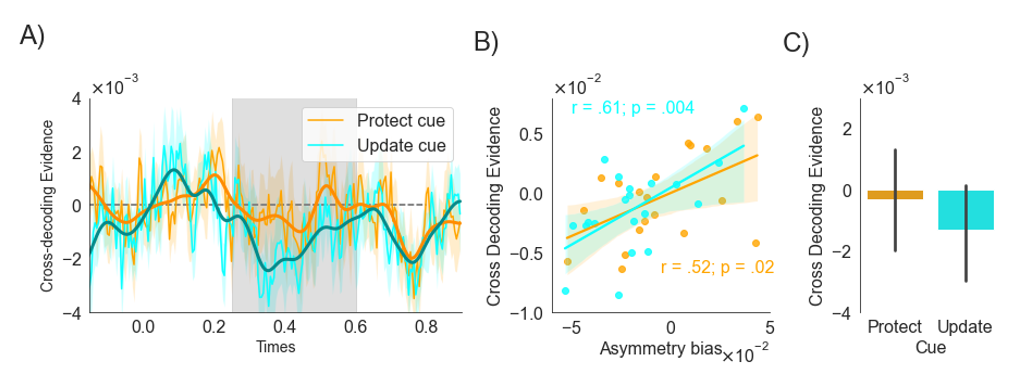
\includegraphics[width=0.9\textwidth]{figures/suppl_fig_crossdec} 
\caption*{\textbf{Supplementary Figure 1: Cross-decoding Evidence for Orientation 1 Upon Presentation of Orientation 2.} A) Cross-decoding after presentation of the second grating orientation on trials where a protect cue (orange) or an update cue (cyan) was presented. Smoothing was applied for visualisation purposes with the same conventions as \textbf{Figure ~\ref{fig:between_decoding}}. The grey-shaded region marks the 250 – 600 ms window used for subplot B-C. B) Scatterplot between neural bias relative to the first orientation presented on the same trial (see results section and \textbf{Figure ~\ref{fig:between_decoding}} for details) and the cross-decoding evidence for the first orientation presented on the same trial. C) Average cross-decoding from 250 – 600 ms. Error bars indicate 95\% confidence intervals. }
\label{fig:suppl_crossdec}
\end{figure}



\end{document}
